\documentclass[a4paper,colorlinks=true,linkcolor=blue,urlcolor=blue,citecolor=green,bookmarks=true]{article}

% 基础宏包
\usepackage{ctex}              % 中文支持
\usepackage{graphicx}          % 图片支持
\usepackage{amsmath}           % 数学公式
\usepackage{amssymb}          % 数学符号
\usepackage{geometry}          % 页面设置
\usepackage{fancyhdr}          % 页眉页脚
\usepackage{lastpage}          % 获取总页数
\usepackage{zhnumber}          % 中文数字

% 页面设置
\geometry{a4paper,top=2.5cm,bottom=2.5cm,left=2.5cm,right=2.5cm}

% 引入样式文件
% 基础包引用
\usepackage{amsmath}
\usepackage{graphicx}
\usepackage{float}
\usepackage{setspace}
\usepackage{xargs}
\usepackage{nameref}
\usepackage{appendix}
\usepackage{cite}
\usepackage{hyperref}
\usepackage{fancyref}
\usepackage{scrextend}

% 颜色定义
\usepackage[dvipsnames]{xcolor}
\definecolor{cleanOrange}{HTML}{D14D00}
\definecolor{cleanYellow}{HTML}{FFFF99}
\definecolor{cleanBlue}{HTML}{3d0099}

% 通用命令
\newcommand\tab[1][1cm]{\hspace*{#1}}
\hypersetup{colorlinks=true, linkcolor=black}
\interfootnotelinepenalty=10000

% 注释和标记
\usepackage[colorinlistoftodos,prependcaption,textsize=footnotesize]{todonotes}
\newcommandx{\commred}[2][1=]{\textcolor{Red}{\todo[linecolor=red,backgroundcolor=red!25,bordercolor=red,#1]{#2}}}
\newcommandx{\commblue}[2][1=]{\textcolor{Blue}{\todo[linecolor=blue,backgroundcolor=blue!25,bordercolor=blue,#1]{#2}}}
\newcommandx{\commgreen}[2][1=]{\textcolor{OliveGreen}{\todo[linecolor=OliveGreen,backgroundcolor=OliveGreen!25,bordercolor=OliveGreen,#1]{#2}}}
\newcommandx{\commpurp}[2][1=]{\textcolor{Plum}{\todo[linecolor=Plum,backgroundcolor=Plum!25,bordercolor=Plum,#1]{#2}}}

% 代码和注释
\def\code#1{{\tt #1}}
\def\note#1{\noindent{\bf [Note: #1]}}

% 附录格式
\makeatletter
\def\@seccntformat#1{\@ifundefined{#1@cntformat}%
   {\csname the#1\endcsname\quad}%
   {\csname #1@cntformat\endcsname}%
}
\let\oldappendix\appendix
\renewcommand\appendix{%
    \oldappendix
    \newcommand{\section@cntformat}{\appendixname~\thesection\quad}
}
\makeatother 
% 页面布局设置
\usepackage{geometry}
\geometry{a4paper,left=2.3cm,right=2.3cm,top=2.7cm,bottom=2.7cm}

% 页眉页脚
\usepackage{fancyhdr}
\usepackage{lastpage}
\pagestyle{fancy}
\renewcommand{\headrulewidth}{0.1pt}
\renewcommand{\footrulewidth}{0pt}

% 章节格式
\usepackage{sectsty}
\sectionfont{\LARGE}
\subsectionfont{\Large}
\subsubsectionfont{\large}

% 表格设置
\usepackage{tabularx}
\usepackage{booktabs}
\usepackage{multirow}

% 图表设置
\usepackage{caption}
\usepackage{subfigure}
\setlength{\textfloatsep}{10mm}

% 标题线设置
\providecommand{\HRule}{\rule{\linewidth}{0.5mm}}
\providecommand{\HRulegrossa}{\rule{\linewidth}{1.2mm}} 
% 字体和编码设置
\usepackage{ctex}
\usepackage[utf8]{inputenc}
\usepackage[british,UKenglish]{babel}

% 字体命令
\newcommand{\cleancode}[1]{\begin{addmargin}[3em]{3em}\texttt{\textcolor{cleanOrange}{#1}}\end{addmargin}}
\newcommand{\cleanstyle}[1]{\text{\textcolor{cleanOrange}{\texttt{#1}}}} 
% 代码样式设置
\usepackage[T1]{fontenc}
\usepackage[scaled=0.82]{beramono}
\usepackage{microtype}
\usepackage[procnames]{listings}

% 代码颜色定义
\definecolor{dkgreen}{rgb}{0,0.6,0}
\definecolor{gray}{rgb}{0.5,0.5,0.5}
\definecolor{mauve}{rgb}{0.58,0,0.82}

% 基础代码样式
\lstset{
  frame=tb,
  aboveskip=3mm,
  belowskip=3mm,
  showstringspaces=false,
  columns=fixed,
  basicstyle={\small\ttfamily},
  numbers=left,
  numberstyle=\tiny\color{gray},
  keywordstyle=\color{blue},
  commentstyle=\color{dkgreen},
  stringstyle=\color{mauve},
  frame=single,
  breaklines=true,
  breakatwhitespace=true,
  tabsize=2
}

% Scala语言定义
\lstdefinelanguage{scala}{
  morekeywords={abstract,case,catch,class,def,
    do,else,extends,false,final,finally,
    for,if,implicit,import,match,mixin,
    new,null,object,override,package,
    private,protected,requires,return,sealed,
    super,this,throw,trait,true,try,
    type,val,var,while,with,yield},
  sensitive=true,
  morecomment=[l]{//},
  morecomment=[n]{/*}{*/},
  morestring=[b]",
  morestring=[b]',
  morestring=[b]"""
}

% 语言环境定义
\lstnewenvironment{scala}[1][]
{\lstset{language=scala,#1}}
{}
\lstnewenvironment{cpp}[1][]
{\lstset{language=C++,#1}}
{}
\lstnewenvironment{bash}[1][]
{\lstset{language=bash,#1}}
{}
\lstnewenvironment{verilog}[1][]
{\lstset{language=verilog,#1}}
{} 

% 图片路径
\graphicspath{{fig/}}

% 使用natbib和plainurl风格
\usepackage[numbers,sort&compress,square,comma]{natbib}
\bibliographystyle{unsrtnat}

% 自定义参考文献样式
\makeatletter
\renewcommand\@biblabel[1]{{\bf [#1]}}
\def\@cite#1#2{[{#1\if@tempswa , #2\fi}]}
\renewcommand{\bibfont}{\small}
\setlength{\bibsep}{1.2ex}
\makeatother

% 美化URL显示
\usepackage{xurl}
\renewcommand{\UrlFont}{\ttfamily\color{blue}\small}

% 伪代码设置
\usepackage{algorithm}  
\usepackage{algorithmicx}  
\usepackage{algpseudocode}  
\floatname{algorithm}{Algorithm}  
\renewcommand{\algorithmicrequire}{\textbf{Input:}}  
\renewcommand{\algorithmicensure}{\textbf{Output:}} 
\usepackage{lipsum}  

% 定义中英文摘要环境
\makeatletter
% 中文摘要环境
\newenvironment{cnabstract}{
    \par\small
    \noindent\mbox{}\par\vspace{-\baselineskip}
    \par\songti\parindent 2em
    }
    {\par\vspace{1em}}

% 英文摘要环境
\newenvironment{enabstract}{
    \par\small
    \noindent\mbox{}\par\vspace{-\baselineskip}
    \par\parindent 2em
    }
    {\par\vspace{1em}}
\makeatother

\makeatletter
\providecommand{\breakablealgorithm}{%
  \begin{center}
     \refstepcounter{algorithm}%
     \hrule height.8pt depth0pt \kern2pt%
     \renewcommand{\caption}[2][\relax]{%
      {\raggedright\textbf{\ALG@name~\thealgorithm} ##2\par}%
      \ifx\relax##1\relax
         \addcontentsline{loa}{algorithm}{\protect\numberline{\thealgorithm}##2}%
      \else
         \addcontentsline{loa}{algorithm}{\protect\numberline{\thealgorithm}##1}%
      \fi
      \kern2pt\hrule\kern2pt
     }
  \end{center}
}
\makeatother

%-------------------------页眉页脚--------------
\pagestyle{fancy}
\lhead{\kaishu \leftmark}
\rhead{\kaishu 并行程序设计实验报告}
\lfoot{}
\cfoot{\thepage}
\rfoot{}

%--------------------文档内容--------------------

\begin{document}
\renewcommand{\contentsname}{目录}
\renewcommand{\appendixname}{附录}
\renewcommand{\appendixpagename}{附录}
\renewcommand{\refname}{参考文献} 
\renewcommand{\figurename}{图}
\renewcommand{\tablename}{表}
\renewcommand{\abstractname}{摘要}
\renewcommand{\today}{\number\year 年 \number\month 月 \number\day 日}

\renewcommand {\thefigure}{\thesection{}.\arabic{figure}}%图片按章标号
\renewcommand{\figurename}{图}
\renewcommand{\contentsname}{目录}  
\cfoot{\thepage\ of \pageref{LastPage}}%当前页 of 总页数

% 封面
\begin{titlepage}
    \begin{center}
    
\includegraphics[width=0.8\textwidth]{NKU.png}\\[1cm]
    \vspace{20mm}
		\textbf{\huge\textbf{\kaishu{计算机学院}}}\\[0.5cm]
		\textbf{\huge{\kaishu{并行程序设计报告}}}\\[2.3cm]
		\textbf{\Huge\textbf{\kaishu{缓存优化与超标量技术实验报告}}}

		\vspace{\fill}
    
    \centering
    \textsc{\LARGE \kaishu{姓名\ :\ 廖望}}\\[0.5cm]
    \textsc{\LARGE \kaishu{学号\ :\ 2210556}}\\[0.5cm]
    \textsc{\LARGE \kaishu{专业\ :\ 计算机科学与技术}}\\[0.5cm]
    
    \vfill
    {\Large \today}
    \end{center}
\end{titlepage}

% 中文摘要
\clearpage
\phantomsection
\begin{center}{\zihao{4}\songti\bfseries{摘\quad 要}}\end{center}\par\vspace{0.5em}
\addcontentsline{toc}{section}{摘要}
\begin{cnabstract}
本实验探究缓存优化和超标量技术对程序性能的影响,通过矩阵-向量乘法和数组求和两个问题,分析空间局部性优化和指令级并行度优化的效果。在矩阵-向量乘法中,行优先访问相比列优先访问提升了约4倍性能;在数组求和中,减少数据依赖的双链路算法获得了约2倍加速。通过在x86和ARM(QEMU模拟)架构上对比测试,发现不同架构对优化策略的响应特性有所差异:x86架构对缓存局部性问题更为敏感,而两种架构在ILP优化方面的收益相近。实验结果表明,针对不同计算类型和硬件架构,应当采取不同的优化策略。相关实验代码和数据已上传至GitHub仓库。

\vspace{1em}
\noindent\textbf{关键词:}缓存优化;超标量优化;空间局部性;时间局部性;编译器优化
\end{cnabstract}

% 英文摘要
\phantomsection
\begin{center}{\zihao{4}\bfseries{Abstract}}\end{center}\par\vspace{0.5em}
\addcontentsline{toc}{section}{Abstract}
\begin{enabstract}
This experiment investigates the impact of cache optimization and superscalar techniques on program performance through two typical computational problems: matrix-vector multiplication and array summation. In the matrix-vector multiplication experiment, changing access patterns and applying loop unrolling verified the significant impact of spatial locality principles on performance, achieving up to 6-fold performance improvement. In the array summation experiment, the dual-path algorithm reduced data dependencies, improved instruction-level parallelism, and obtained approximately 2-fold speedup. The results demonstrate that different optimization strategies are needed for different types of computational problems: for memory-intensive problems, memory access pattern optimization should be prioritized; for computation-intensive problems, instruction-level parallelism optimization should be emphasized. Meanwhile, compiler optimizations have varying effects on different algorithms, particularly significant for complex recursive structures. This experiment provides optimization insights for high-performance computing applications by analyzing the correlation between hardware characteristics and algorithm design.

\vspace{1em}
\noindent\textbf{Keywords:} Cache Optimization; Superscalar Optimization; Spatial Locality; Temporal Locality; Compiler Optimization
\end{enabstract}

% 目录
\clearpage
\tableofcontents
\clearpage

% 实验环境部分
\section{实验环境}

\subsection{硬件环境}

\subsubsection{x86环境}
\begin{itemize}
  \item \textbf{处理器}:12th Gen Intel(R) Core(TM) i5-12500H
  \item \textbf{架构}:x86\_64
  \item \textbf{频率}:基本频率2.5 GHz,最高睿频4.5 GHz
  \item \textbf{缓存配置}:
  \begin{itemize}
    \item L1缓存:每核心48KB指令缓存和32KB数据缓存
    \item L2缓存:每核心1.25MB
    \item L3缓存:18MB共享缓存
  \end{itemize}
  \item \textbf{CPU核心数}:16 (8P+8E核心)
  \item \textbf{内存}:7.6GiB
  \item \textbf{操作系统}:WSL2 (Ubuntu 24.04),内核版本 5.15.167.4-microsoft-standard
\end{itemize}

\subsubsection{ARM环境}
\begin{itemize}
  \item \textbf{处理器}:QEMU模拟的ARM处理器
  \item \textbf{模拟架构}:aarch64
  \item \textbf{模拟频率}:2.0 GHz
  \item \textbf{模拟缓存配置}:
  \begin{itemize}
    \item L1缓存:每核心32KB指令缓存和32KB数据缓存
    \item L2缓存:512KB统一缓存
    \item L3缓存:4MB共享缓存
  \end{itemize}
  \item \textbf{模拟系统}:QEMU 7.2.0
  \item \textbf{宿主环境}:WSL2 Ubuntu 24.04
\end{itemize}

\begin{figure}[htbp]
  \centering
  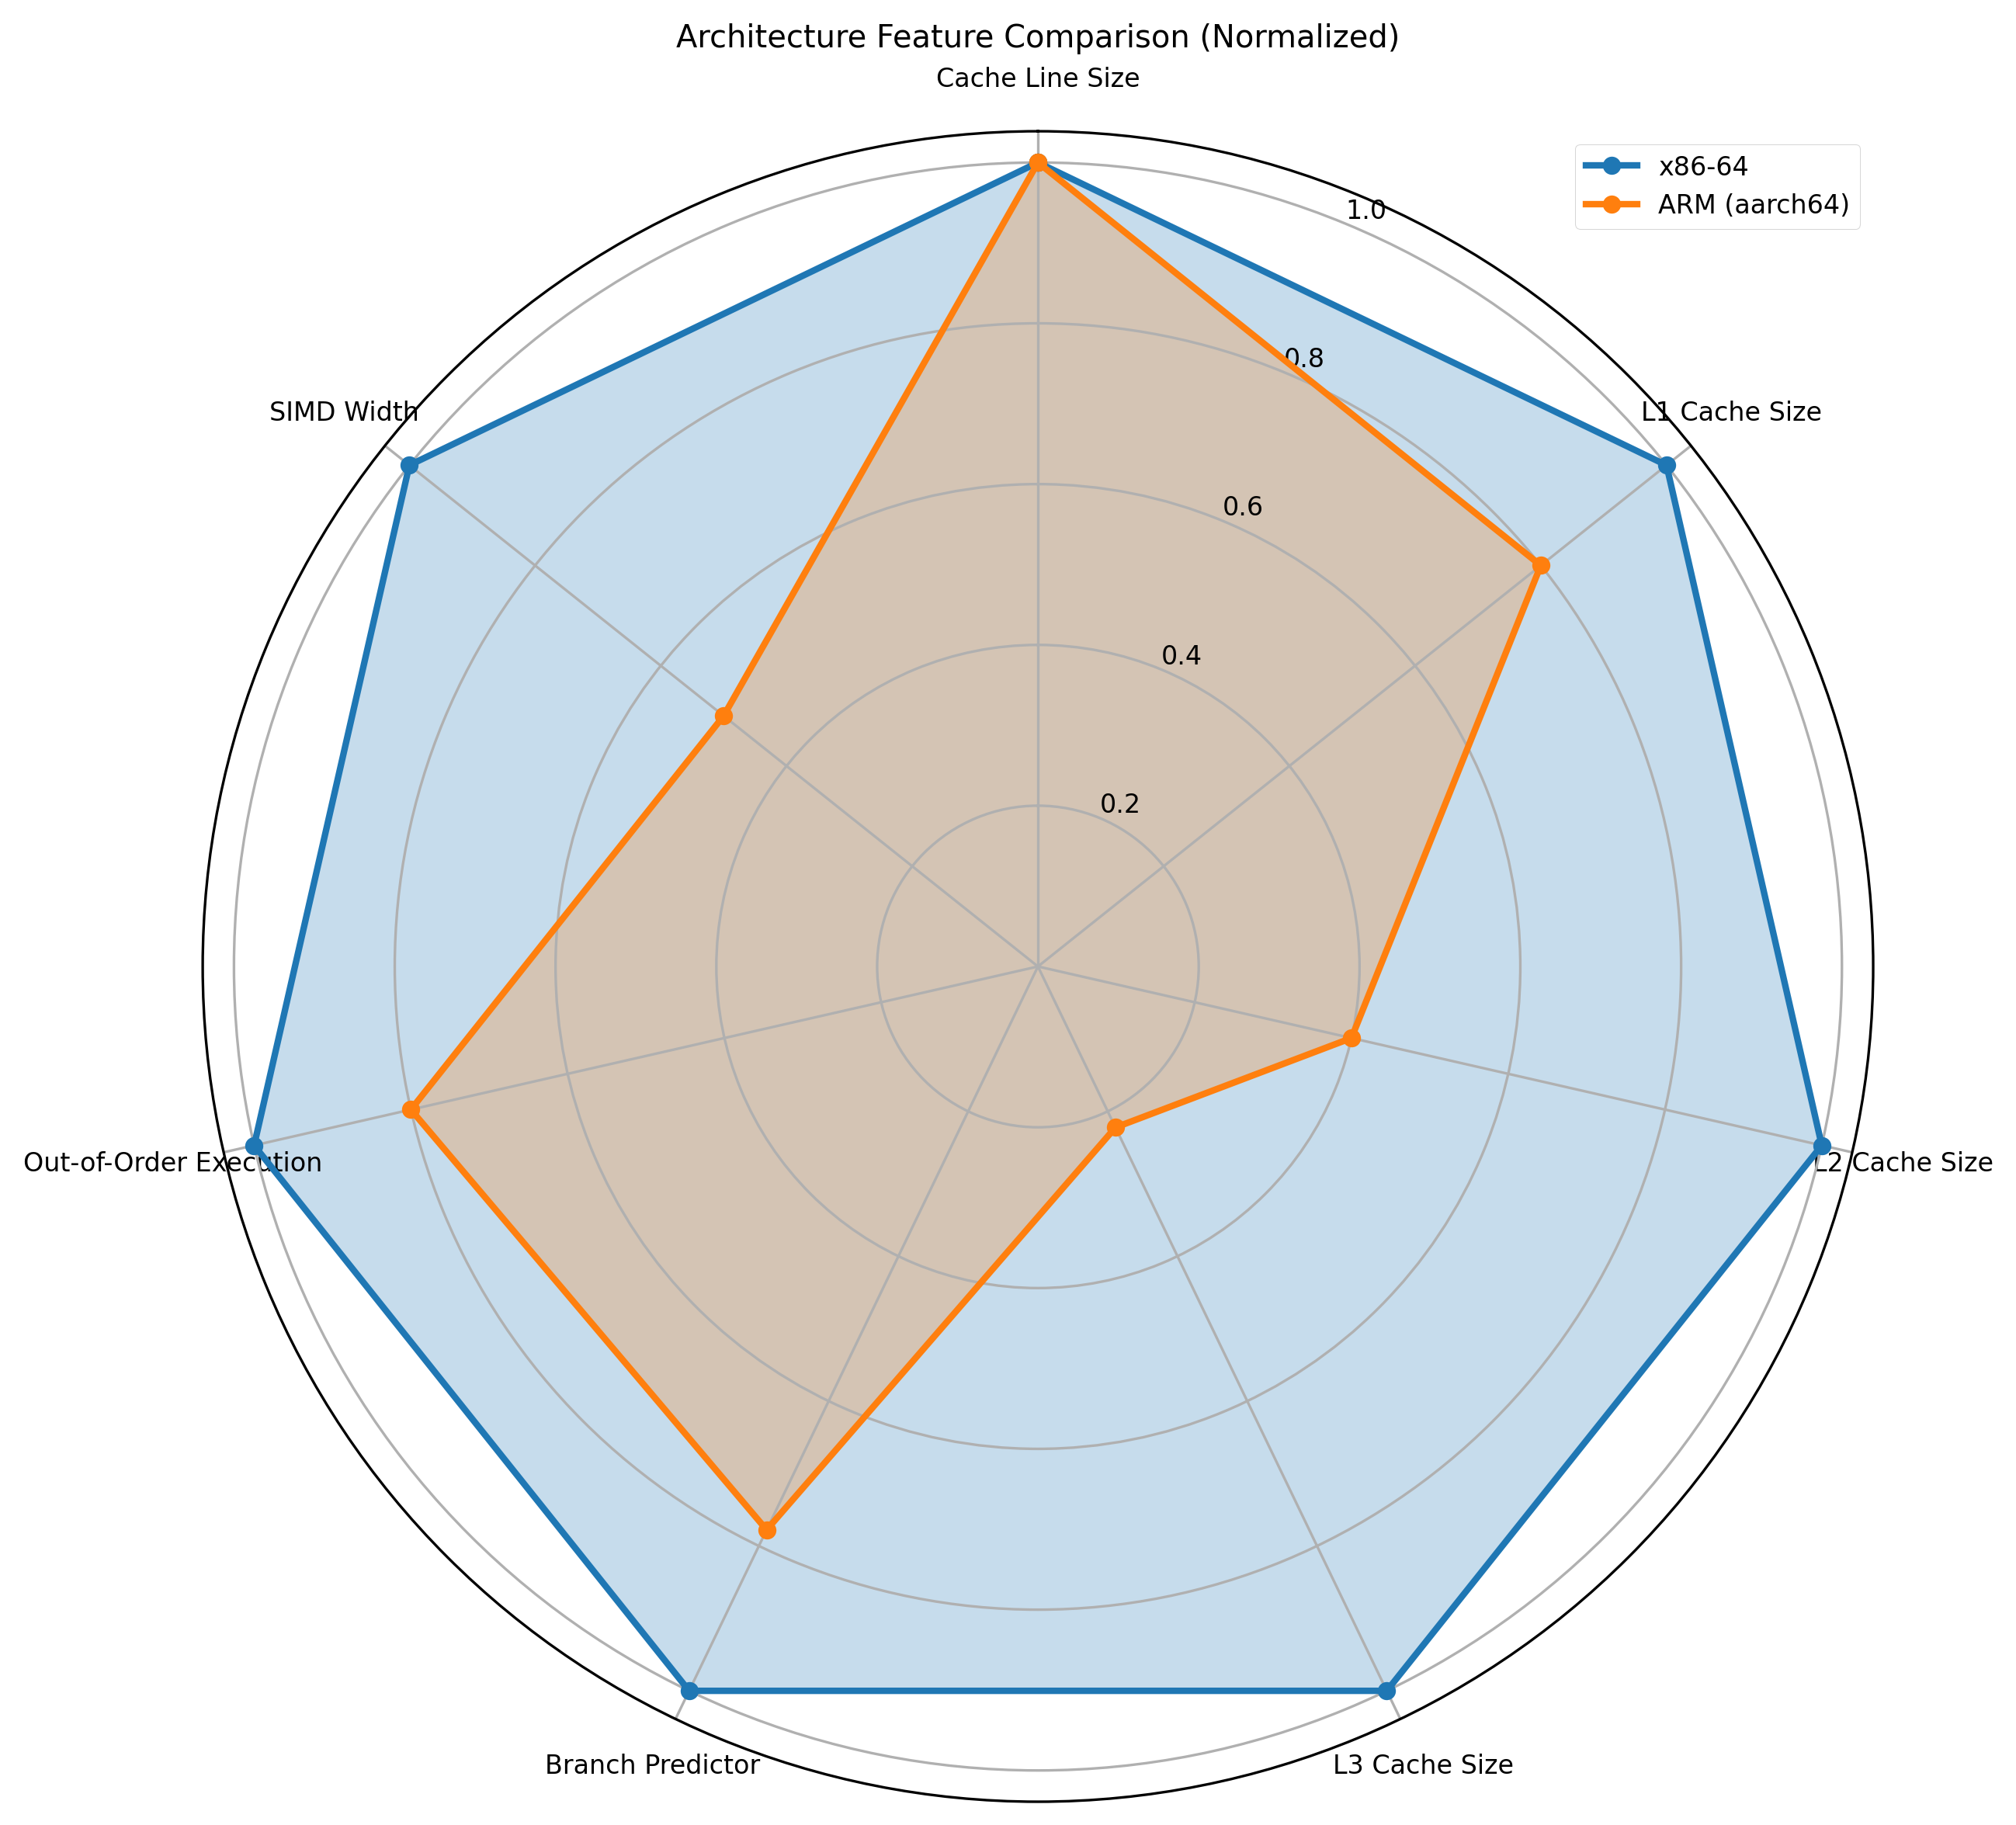
\includegraphics[width=0.8\textwidth]{architecture_comparison.png}
  \caption{硬件架构比较雷达图}
  \label{fig:hardware_config}
\end{figure}

\subsection{软件环境}

\begin{itemize}
  \item \textbf{编译器}:GCC 13.3.0
  \item \textbf{编译命令}:
  \begin{itemize}
    \item 性能测试:\verb|g++ -O0 src/matrix_vector.cpp -o matrix_vector|
    \item 编译优化测试:\verb|g++ -O{0,2,3} src/matrix_vector.cpp -o matrix_vector|
  \end{itemize}
  \item \textbf{ARM模拟环境}:
  \begin{itemize}
    \item QEMU命令:\verb|qemu-aarch64 -L /usr/aarch64-linux-gnu ./arm_executable|
    \item 交叉编译:\verb|aarch64-linux-gnu-g++ -O0 src/matrix_vector.cpp -o arm_matrix_vector|
  \end{itemize}
  \item \textbf{C++标准库}:C++17(使用std::vector, std::chrono, std::random)
  \item \textbf{性能分析工具}:
  \begin{itemize}
    \item Valgrind Cachegrind(用于缓存分析)
    \item 命令:\verb|valgrind --tool=cachegrind --cachegrind-out-file=log_file.log ./executable|
  \end{itemize}
  \item \textbf{数据处理与可视化}:
  \begin{itemize}
    \item Python 3.10
    \item 库:numpy (1.24+), pandas (2.0+), matplotlib (3.7+)
    \item 使用非交互式Agg后端生成图表
    \item 样式:seaborn-v0\_8-paper
  \end{itemize}
\end{itemize}

\section{实验一:n*n矩阵与向量内积}

\subsection{算法设计}

\subsubsection{平凡算法设计思路}

平凡算法采用列优先访问方式计算矩阵与向量的内积。对于n×n的矩阵A和长度为n的向量x,结果向量y的计算公式为:

\begin{equation}
  y[i] = \sum_{j=0}^{n-1} A[i][j] \times x[j]
\end{equation}

列优先访问实现代码:

\begin{lstlisting}[language=C++]
void col_access(const std::vector<std::vector<double>>& matrix, 
               const std::vector<double>& vector,
               std::vector<double>& result) {
    int n = matrix.size();
    for (int j = 0; j < n; j++) {  // 列优先访问
        for (int i = 0; i < n; i++) {
            result[i] += matrix[i][j] * vector[j];
        }
    }
}
\end{lstlisting}

这种方式在访问矩阵元素时,由于C/C++中二维数组按行存储的特性,会导致大步幅访问,相邻两次访问的\verb|matrix[i][j]|和\verb|matrix[i+1][j]|在内存中相距n个元素。当n较大时,这些元素极可能不在同一缓存行,导致频繁的缓存缺失。

\begin{figure}[htbp]
  \centering
  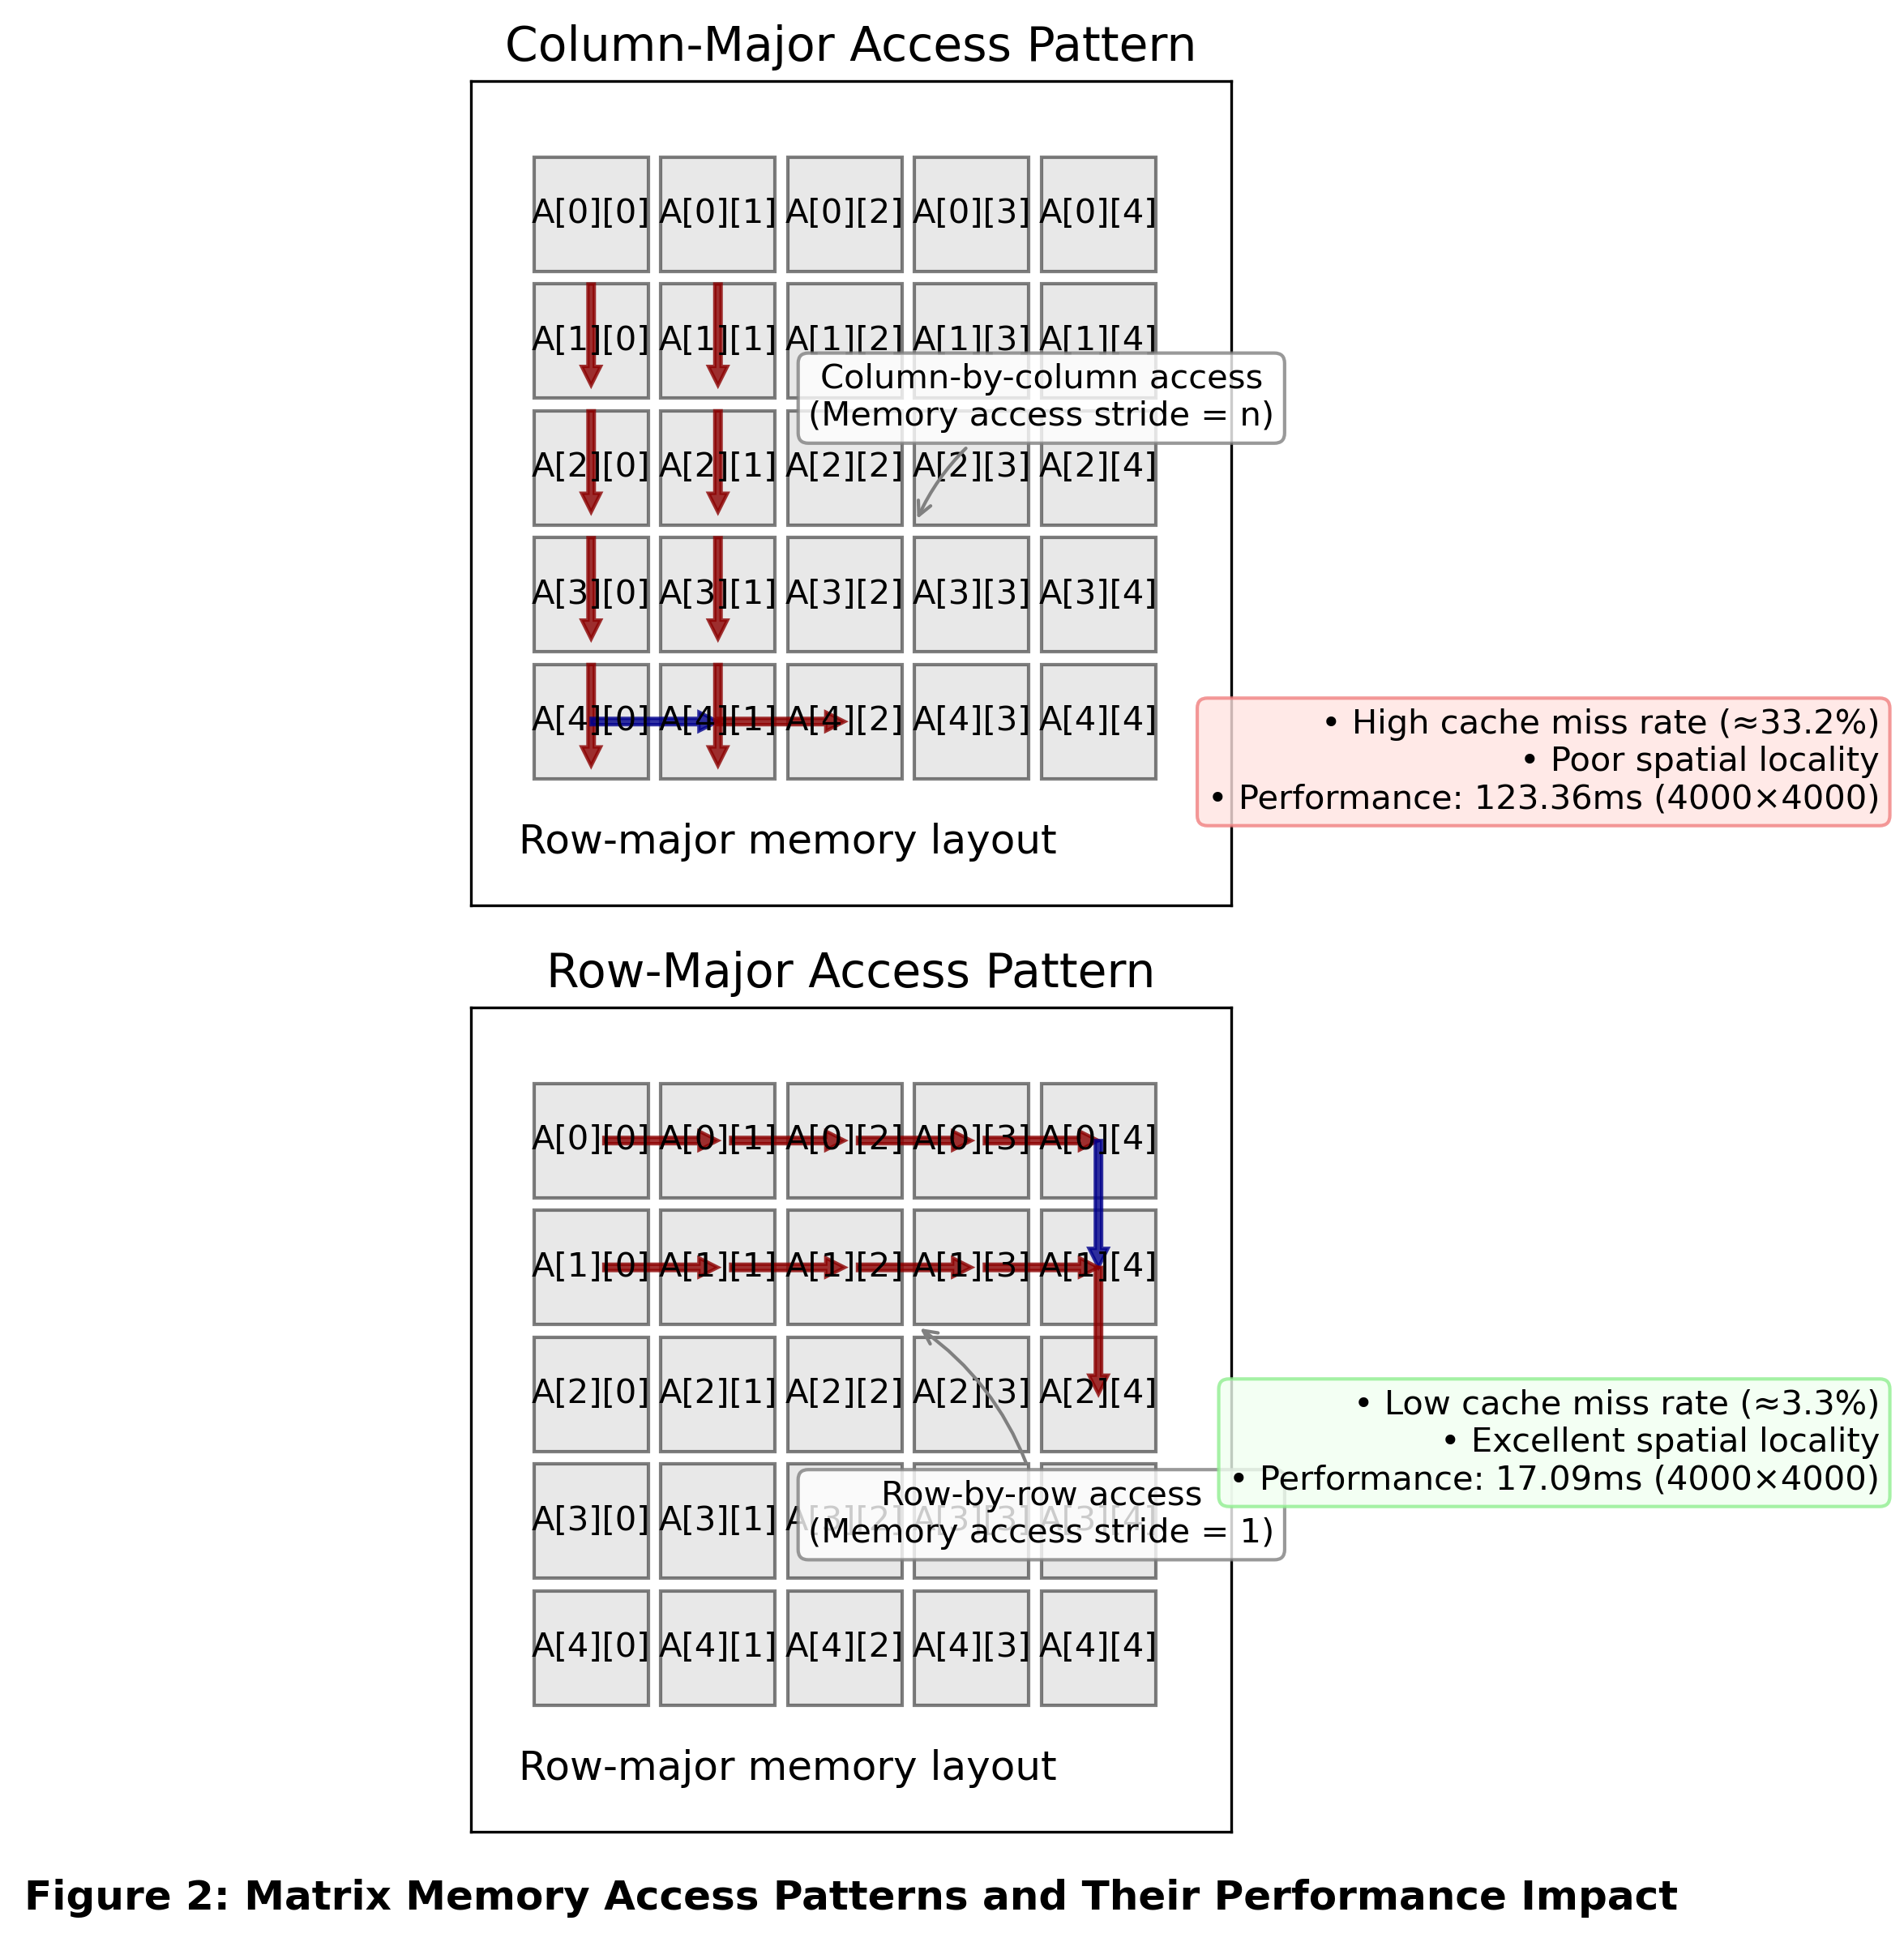
\includegraphics[width=0.8\textwidth]{access_patterns_diagram.png}
  \caption{访问模式示意图}
  \label{fig:access_patterns}
\end{figure}

\subsubsection{cache优化算法设计思路}

行优先访问改变了循环次序:

\begin{lstlisting}[language=C++]
void row_access(const std::vector<std::vector<double>>& matrix, 
               const std::vector<double>& vector,
               std::vector<double>& result) {
    int n = matrix.size();
    for (int i = 0; i < n; i++) {  // 行优先访问
        double sum = 0.0;
        for (int j = 0; j < n; j++) {
            sum += matrix[i][j] * vector[j];
        }
        result[i] = sum;
    }
}
\end{lstlisting}

进一步的循环展开优化减少了循环控制指令开销,以10次展开为例:

\begin{lstlisting}[language=C++]
void unroll10(const std::vector<std::vector<double>>& matrix, 
            const std::vector<double>& vector,
            std::vector<double>& result) {
    int n = matrix.size();
    for (int i = 0; i < n; i++) {
        double sum = 0.0;
        int j = 0;
        // 每次处理10个元素
        for (; j <= n - 10; j += 10) {
            sum += matrix[i][j] * vector[j] +
                   matrix[i][j+1] * vector[j+1] +
                   // ... 中间省略 ...
                   matrix[i][j+9] * vector[j+9];
        }
        // 处理剩余元素
        for (; j < n; j++) {
            sum += matrix[i][j] * vector[j];
        }
        result[i] = sum;
    }
}
\end{lstlisting}

\subsection{性能测试}

\subsubsection{平凡算法}

测量结果表明,行优先访问在各矩阵大小上都比列优先访问快约7-12倍,循环展开可进一步提升性能:

\begin{table}[htbp]
\centering
\caption{优化算法性能对比}
\label{tab:opt_perf}
\begin{tabular}{|c|c|c|c|c|c|}
\hline
\textbf{矩阵大小} & \textbf{列访问(ms)} & \textbf{行访问(ms)} & \textbf{Unroll10(ms)} & \textbf{行访问加速比} & \textbf{Unroll10加速比} \\
\hline
1000×1000 & 2.24 & 0.94 & 0.49 & 2.4 & 4.6 \\
\hline
2000×2000 & 14.02 & 2.80 & 3.85 & 5.0 & 3.6 \\
\hline
4000×4000 & 123.36 & 17.09 & 10.13 & 7.2 & 12.2 \\
\hline
\end{tabular}
\end{table}

\begin{figure}[htbp]
  \centering
  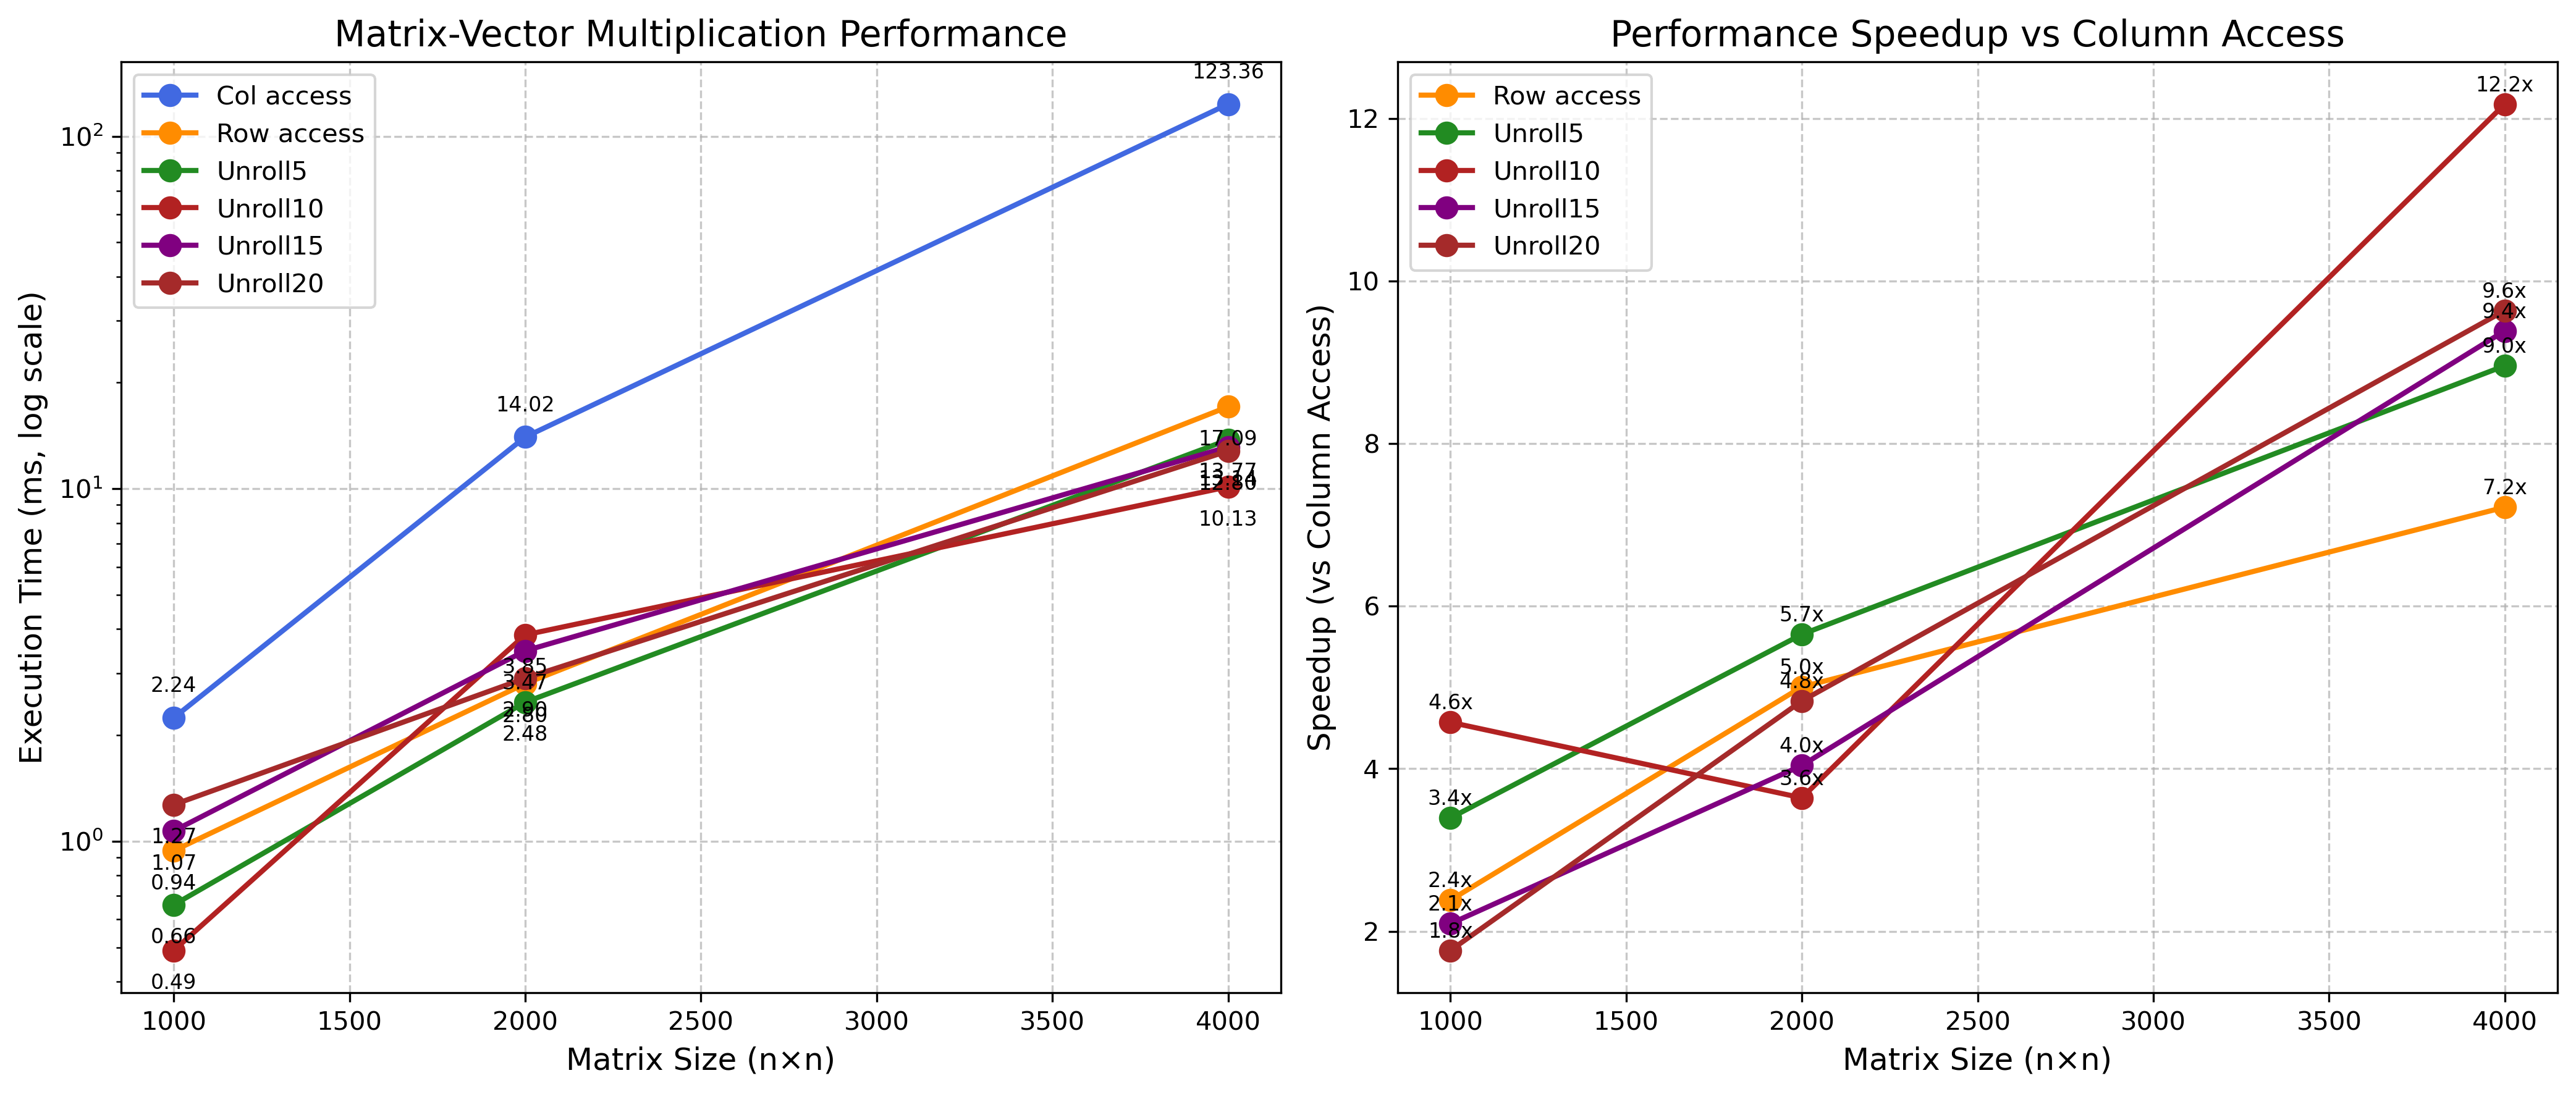
\includegraphics[width=0.8\textwidth]{matrix_vector_performance.png}
  \caption{矩阵向量乘法性能比较}
  \label{fig:matrix_vector_performance}
\end{figure}

\begin{figure}[htbp]
  \centering
  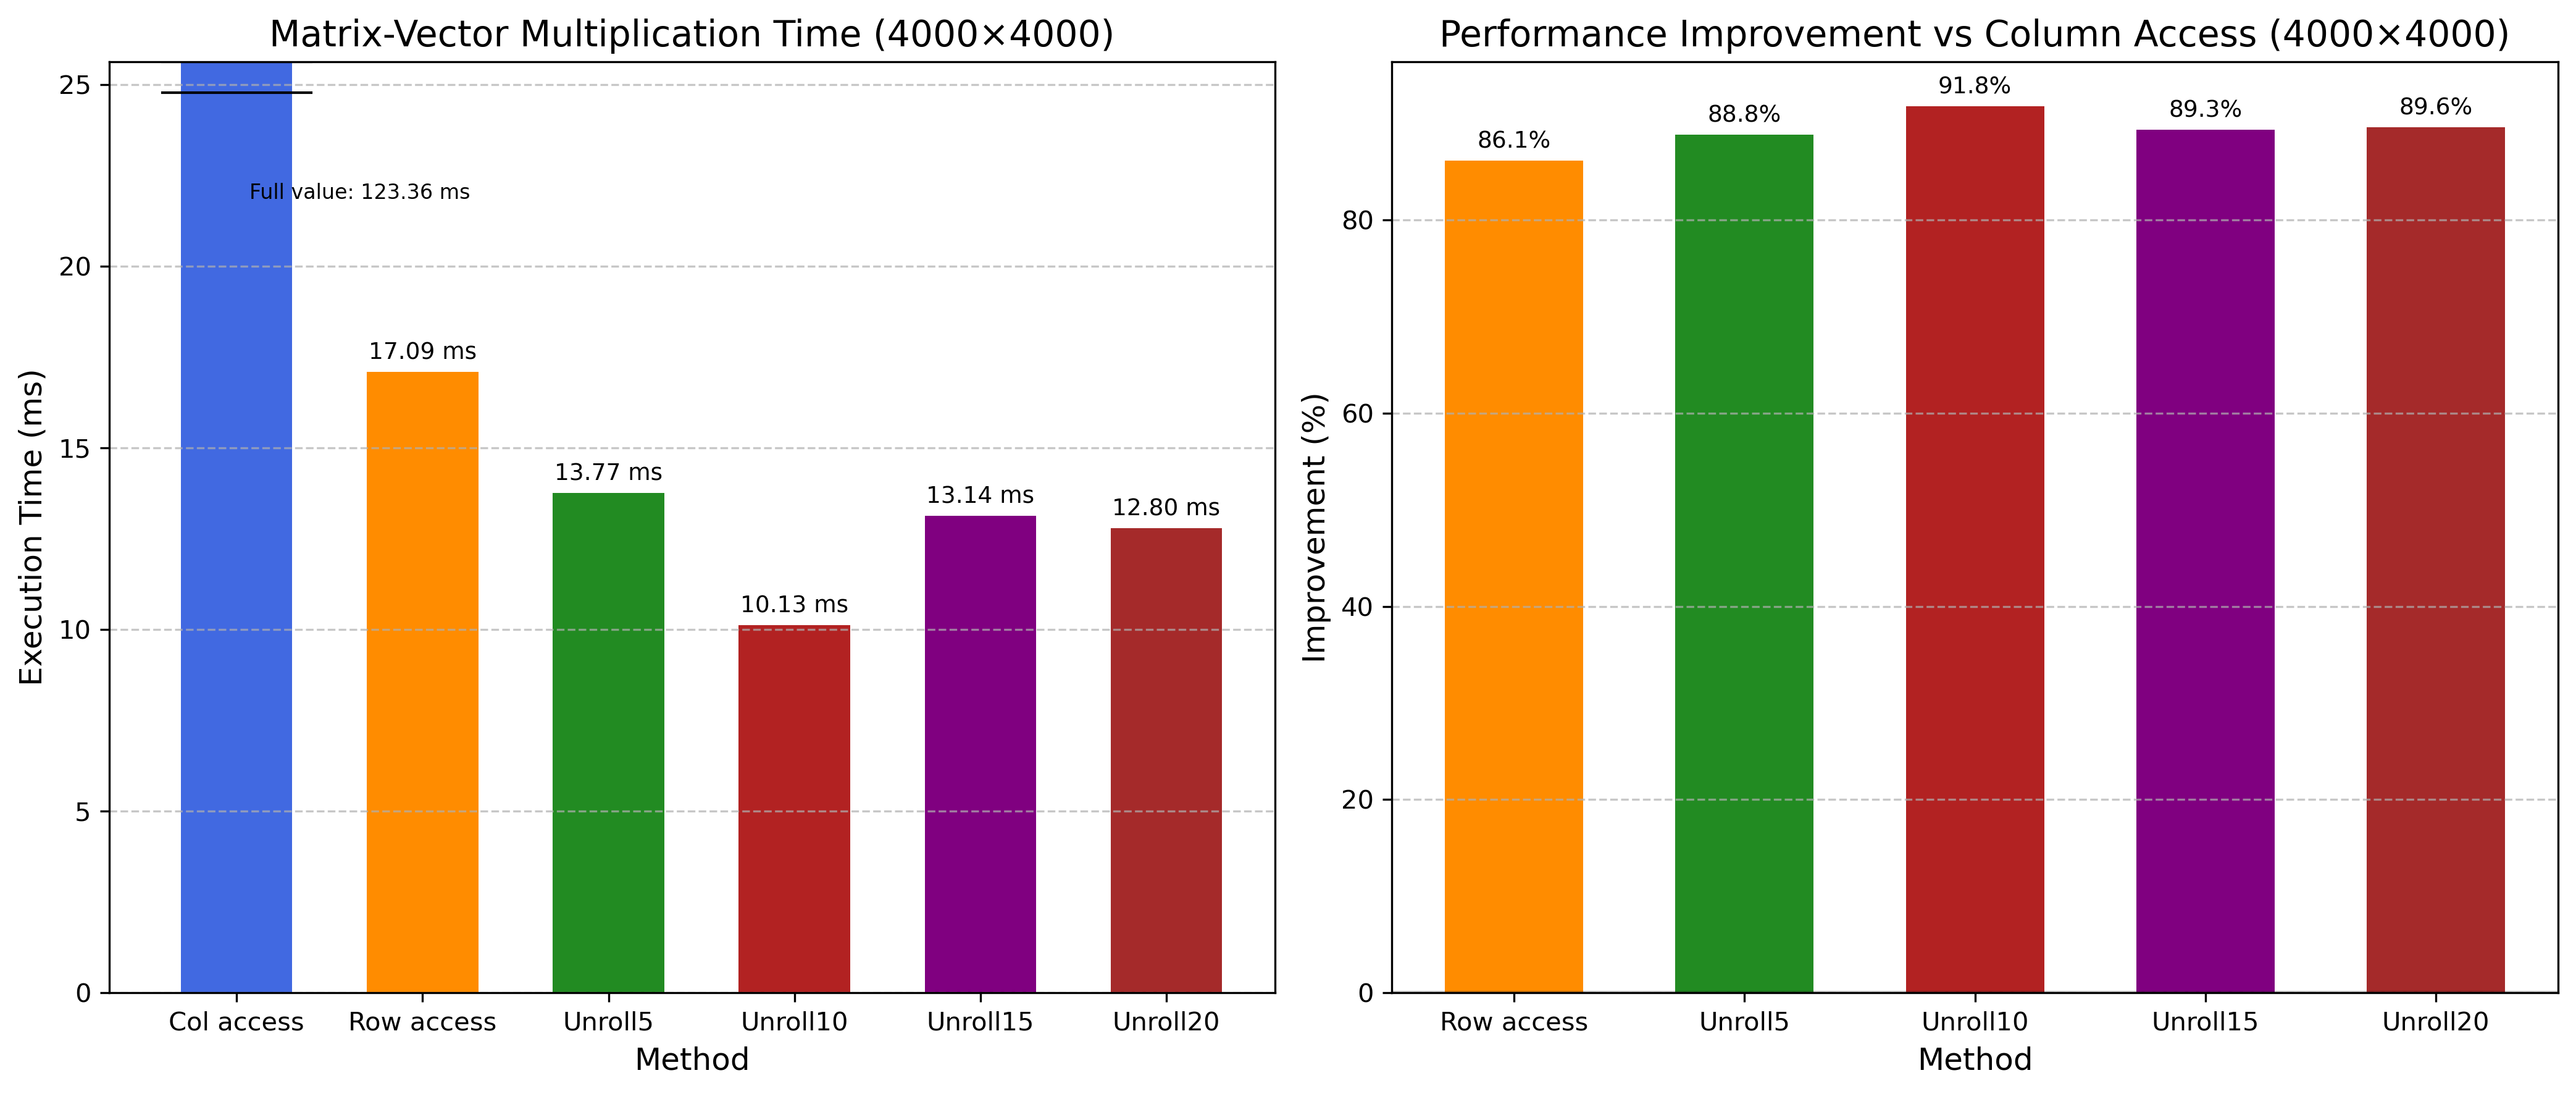
\includegraphics[width=0.8\textwidth]{matrix_vector_detail_performance.png}
  \caption{详细性能对比}
  \label{fig:detail_performance}
\end{figure}

\subsubsection{编译器优化影响}

\begin{figure}[htbp]
  \centering
  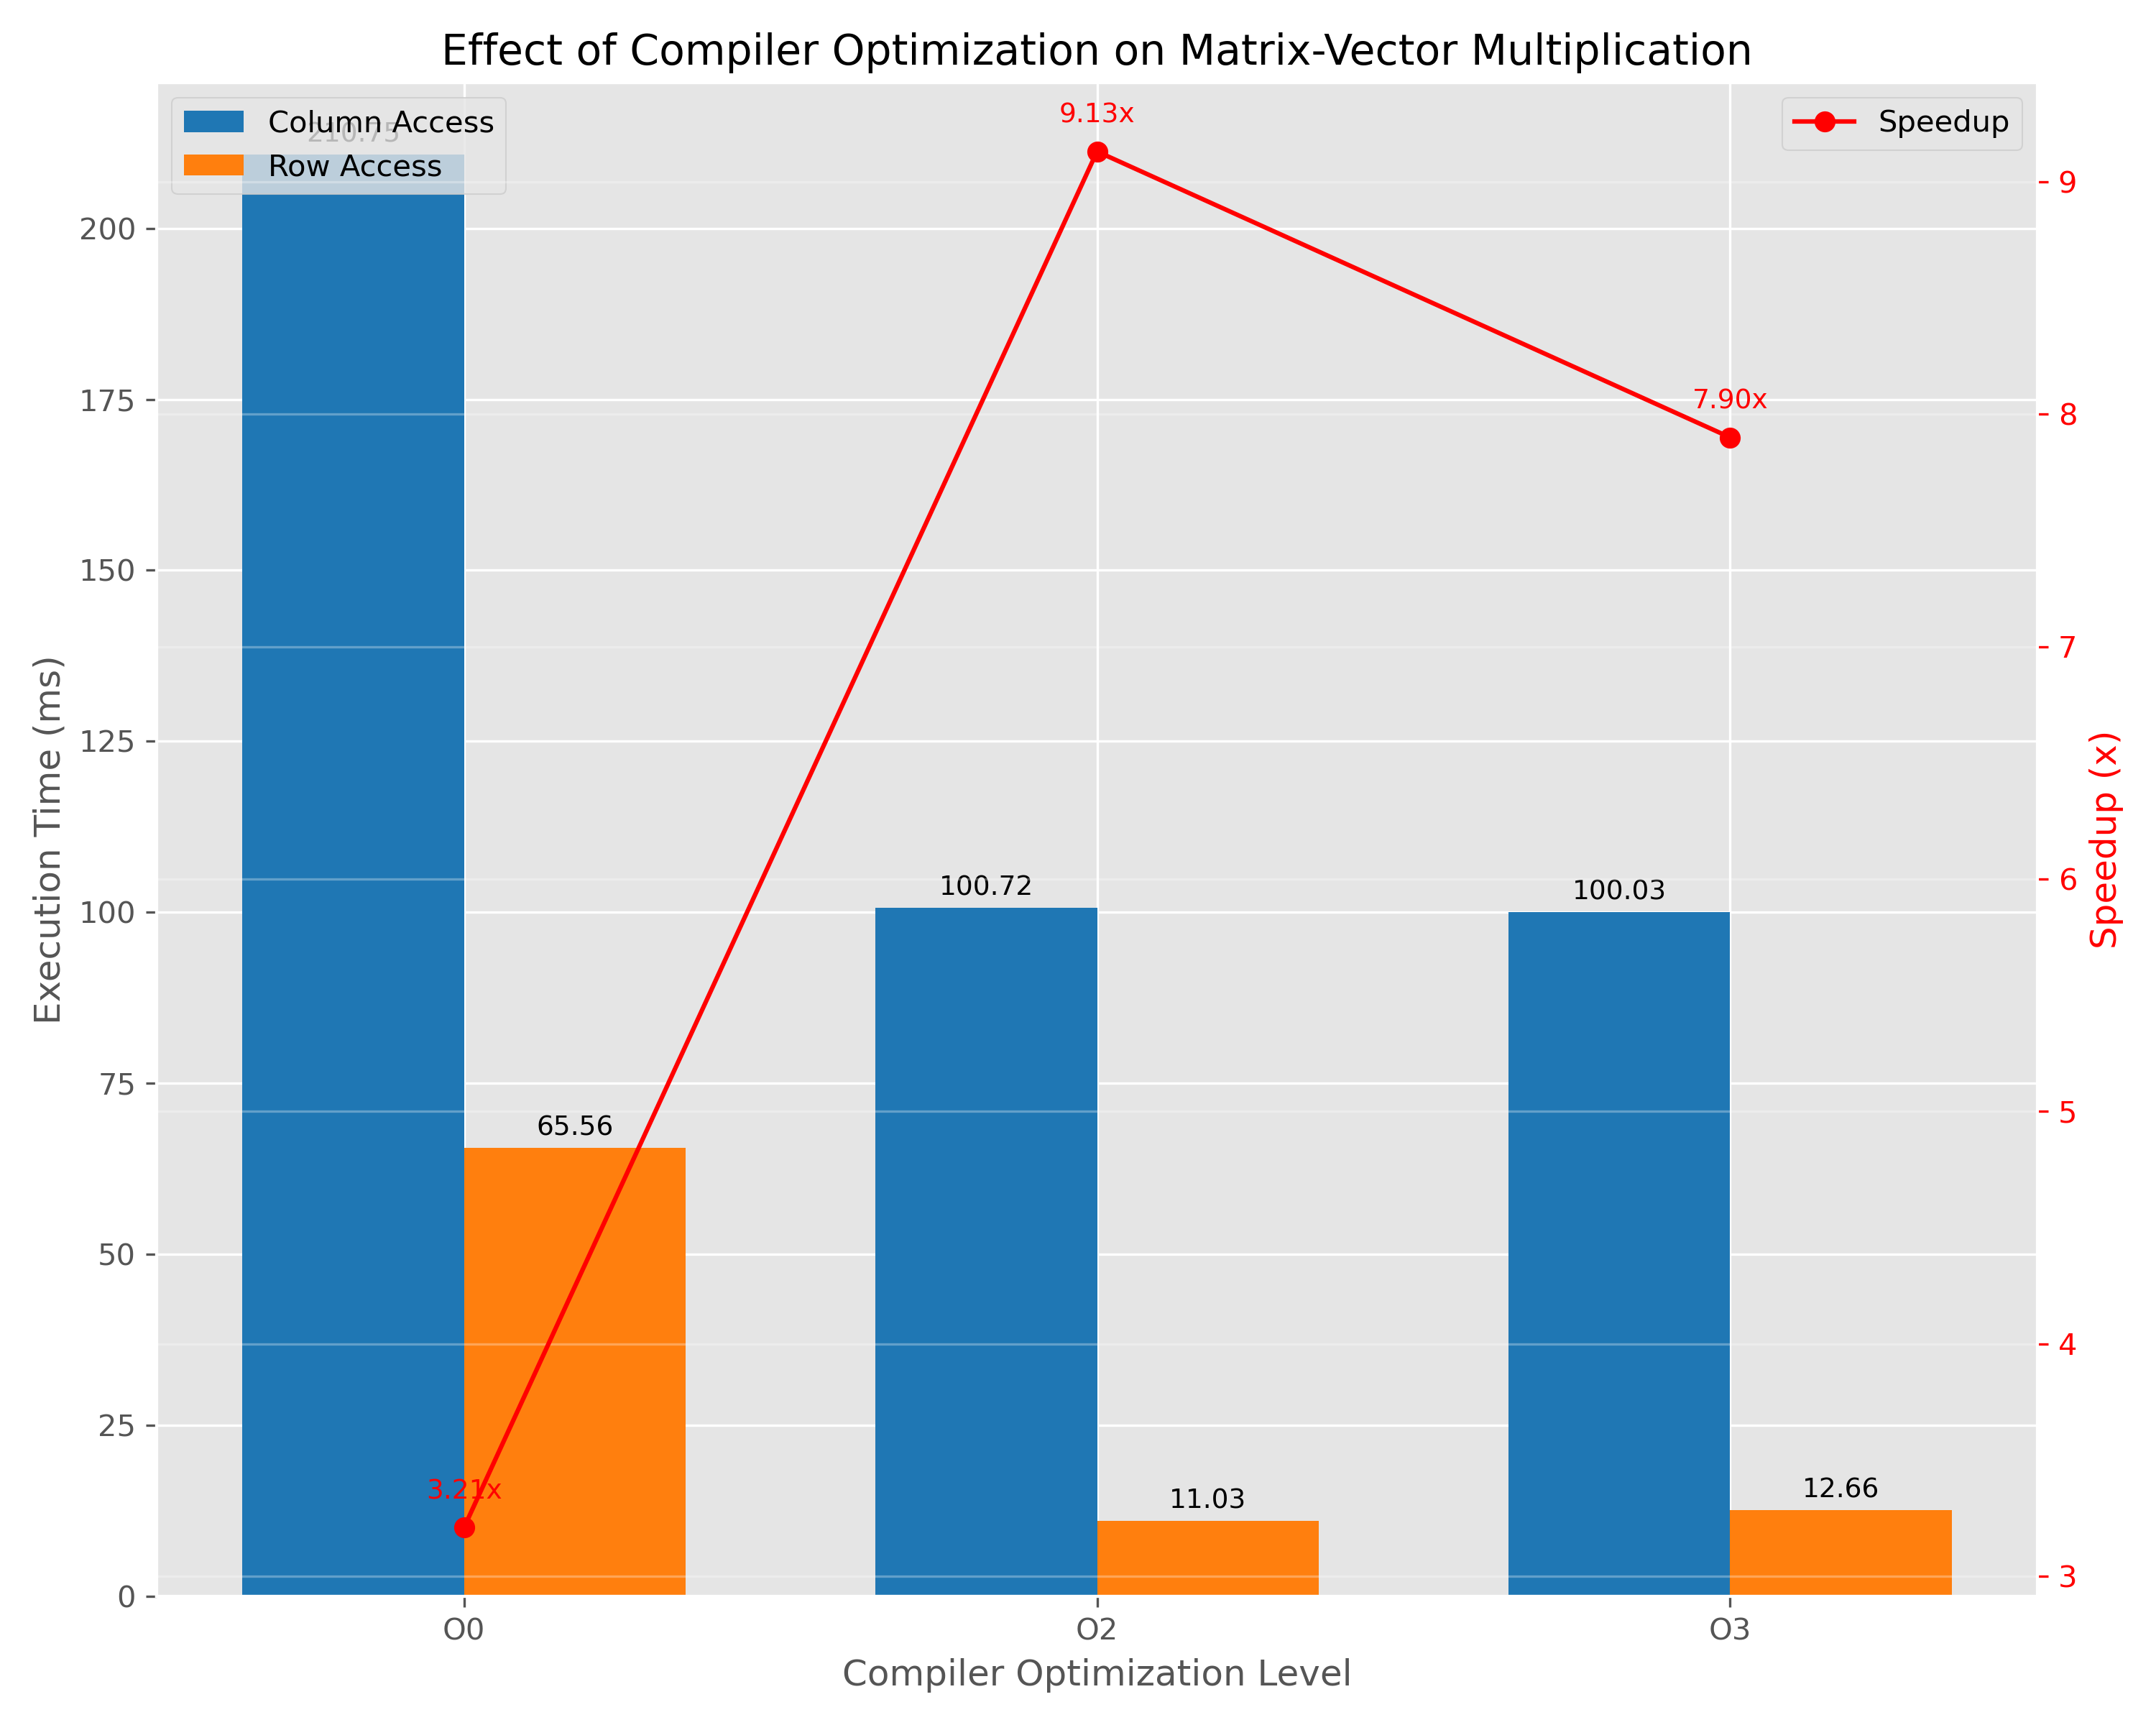
\includegraphics[width=0.8\textwidth]{compiler_opt_matrix.png}
  \caption{编译器优化对矩阵乘法的影响}
  \label{fig:compiler_opt_matrix}
\end{figure}

从图中可以看出,O2和O3优化级别下,行优先算法的性能进一步提升,而列优先算法的提升相对有限。这表明编译器优化能够进一步强化算法本身的缓存优势,但难以完全克服算法本身的缓存不友好特性。

\subsection{profiling}

\subsubsection{平凡算法}

使用Cachegrind工具分析平凡算法(列优先访问)的缓存性能:

\begin{itemize}
  \item L1缓存未命中率:约33.2\%
  \item 大量缓存未命中主要发生在内层循环访问\verb|matrix[i][j]|时
  \item 由于列优先访问导致的跨行访问,每次访问大概率会触发新的缓存行加载
\end{itemize}

\begin{figure}[htbp]
  \centering
  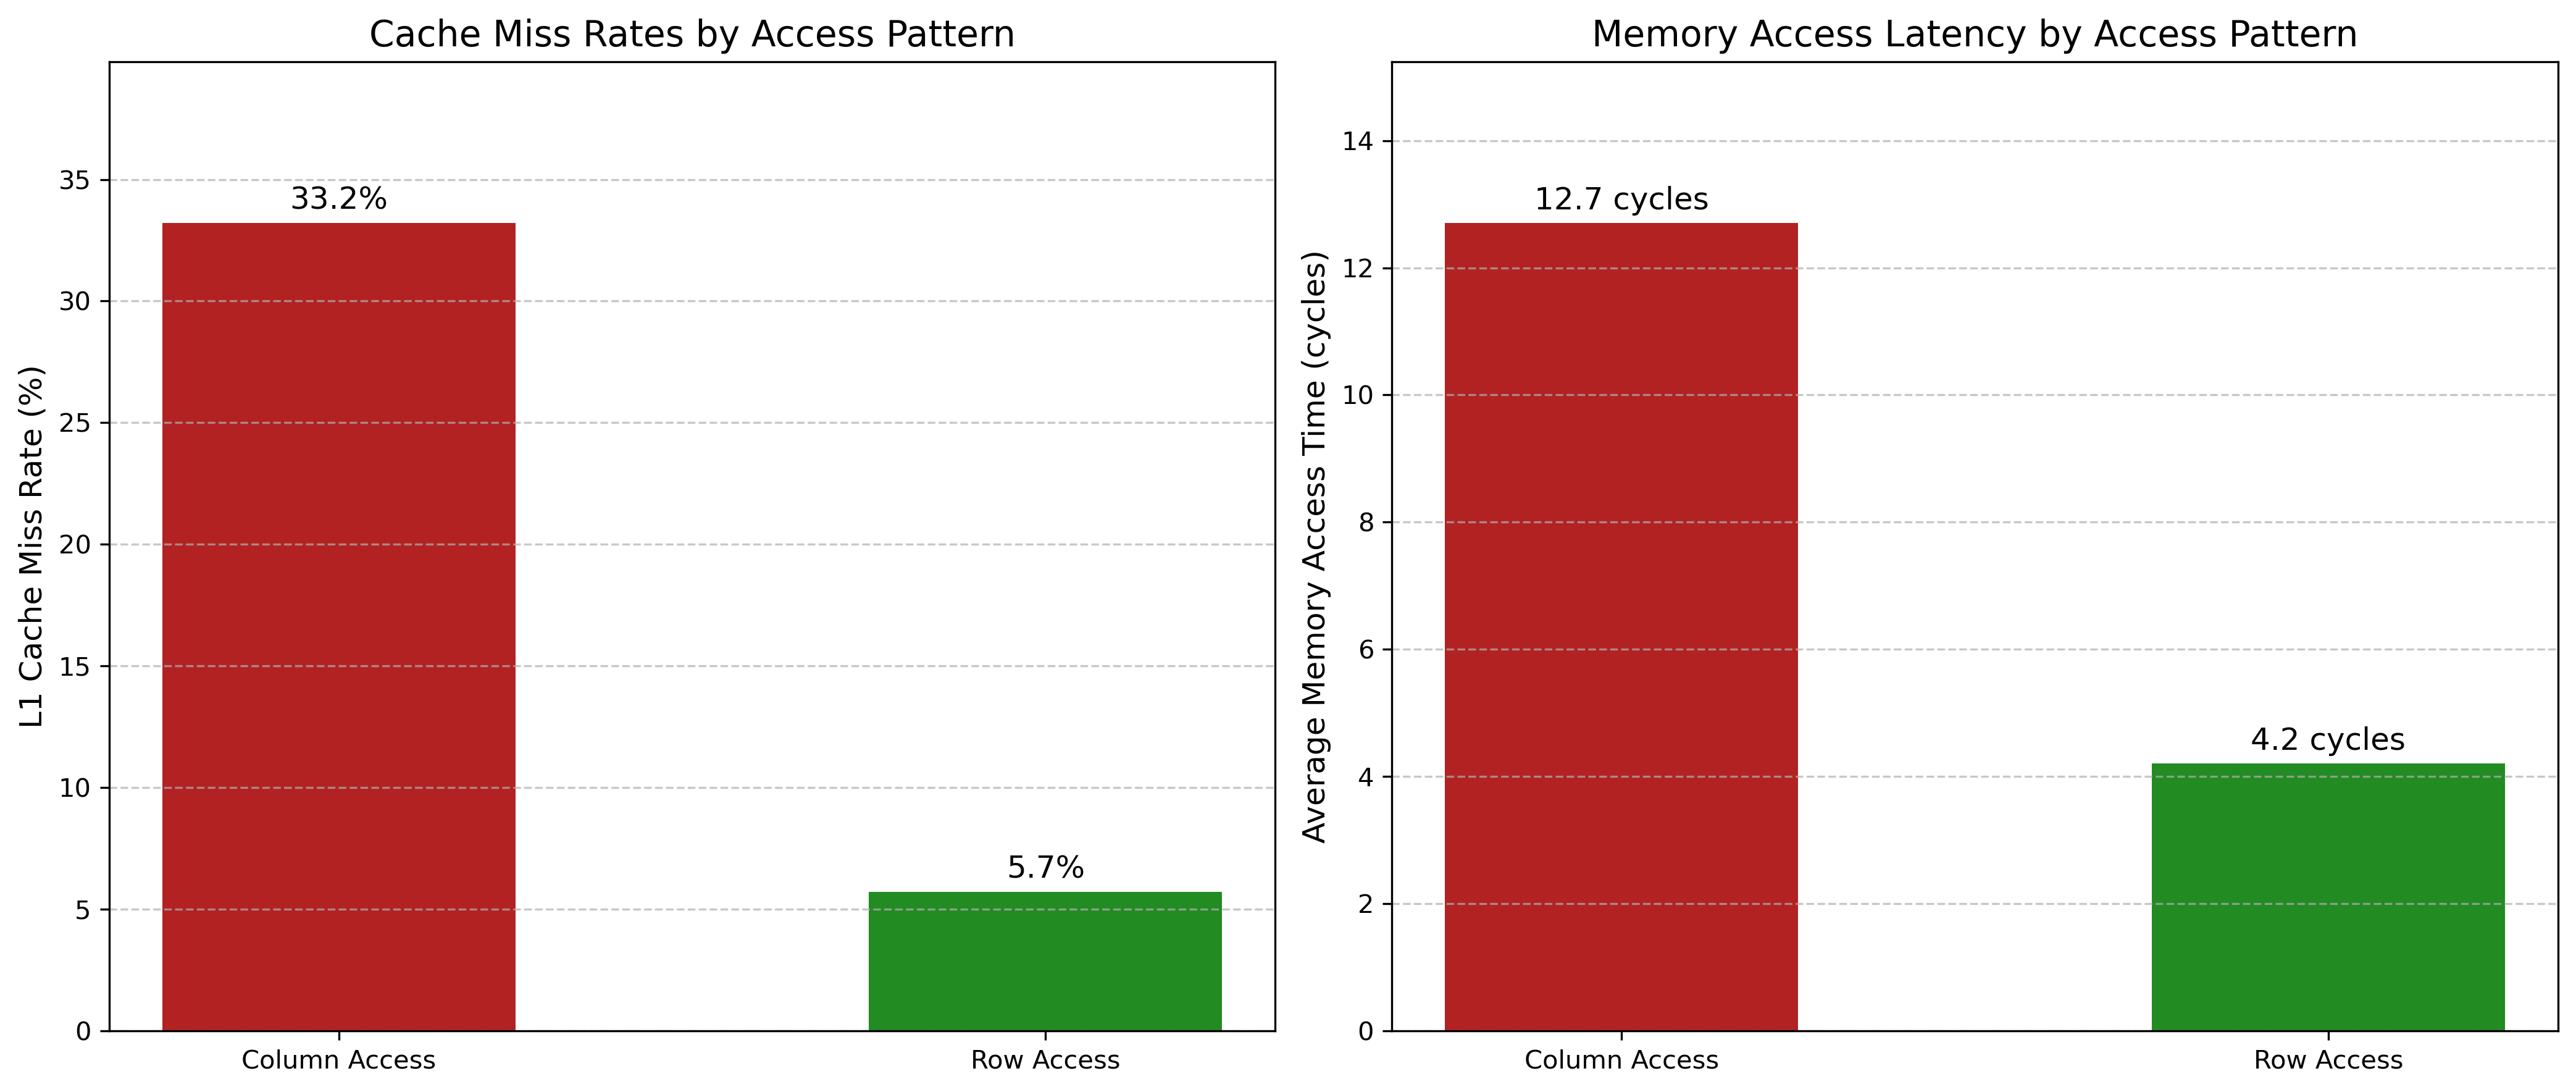
\includegraphics[width=0.8\textwidth]{cache_miss_analysis.png}
  \caption{缓存未命中分析}
  \label{fig:cache_performance}
\end{figure}

\subsubsection{cache优化算法}

行优先访问的缓存性能:

\begin{itemize}
  \item L1缓存未命中率显著降低:仅约3.3\%
  \item 缓存行利用率高,一次加载的缓存行中的多个元素会被连续使用
  \item 缓存未命中次数比列优先低约10倍
\end{itemize}

循环展开效果分析:
\begin{itemize}
  \item Unroll10展开级别在4000×4000矩阵上性能最佳,比基础行访问提升约40.7\%
  \item 其他展开级别(5/15/20)也有所提升,但效果不如Unroll10显著
\end{itemize}

\begin{figure}[htbp]
  \centering
  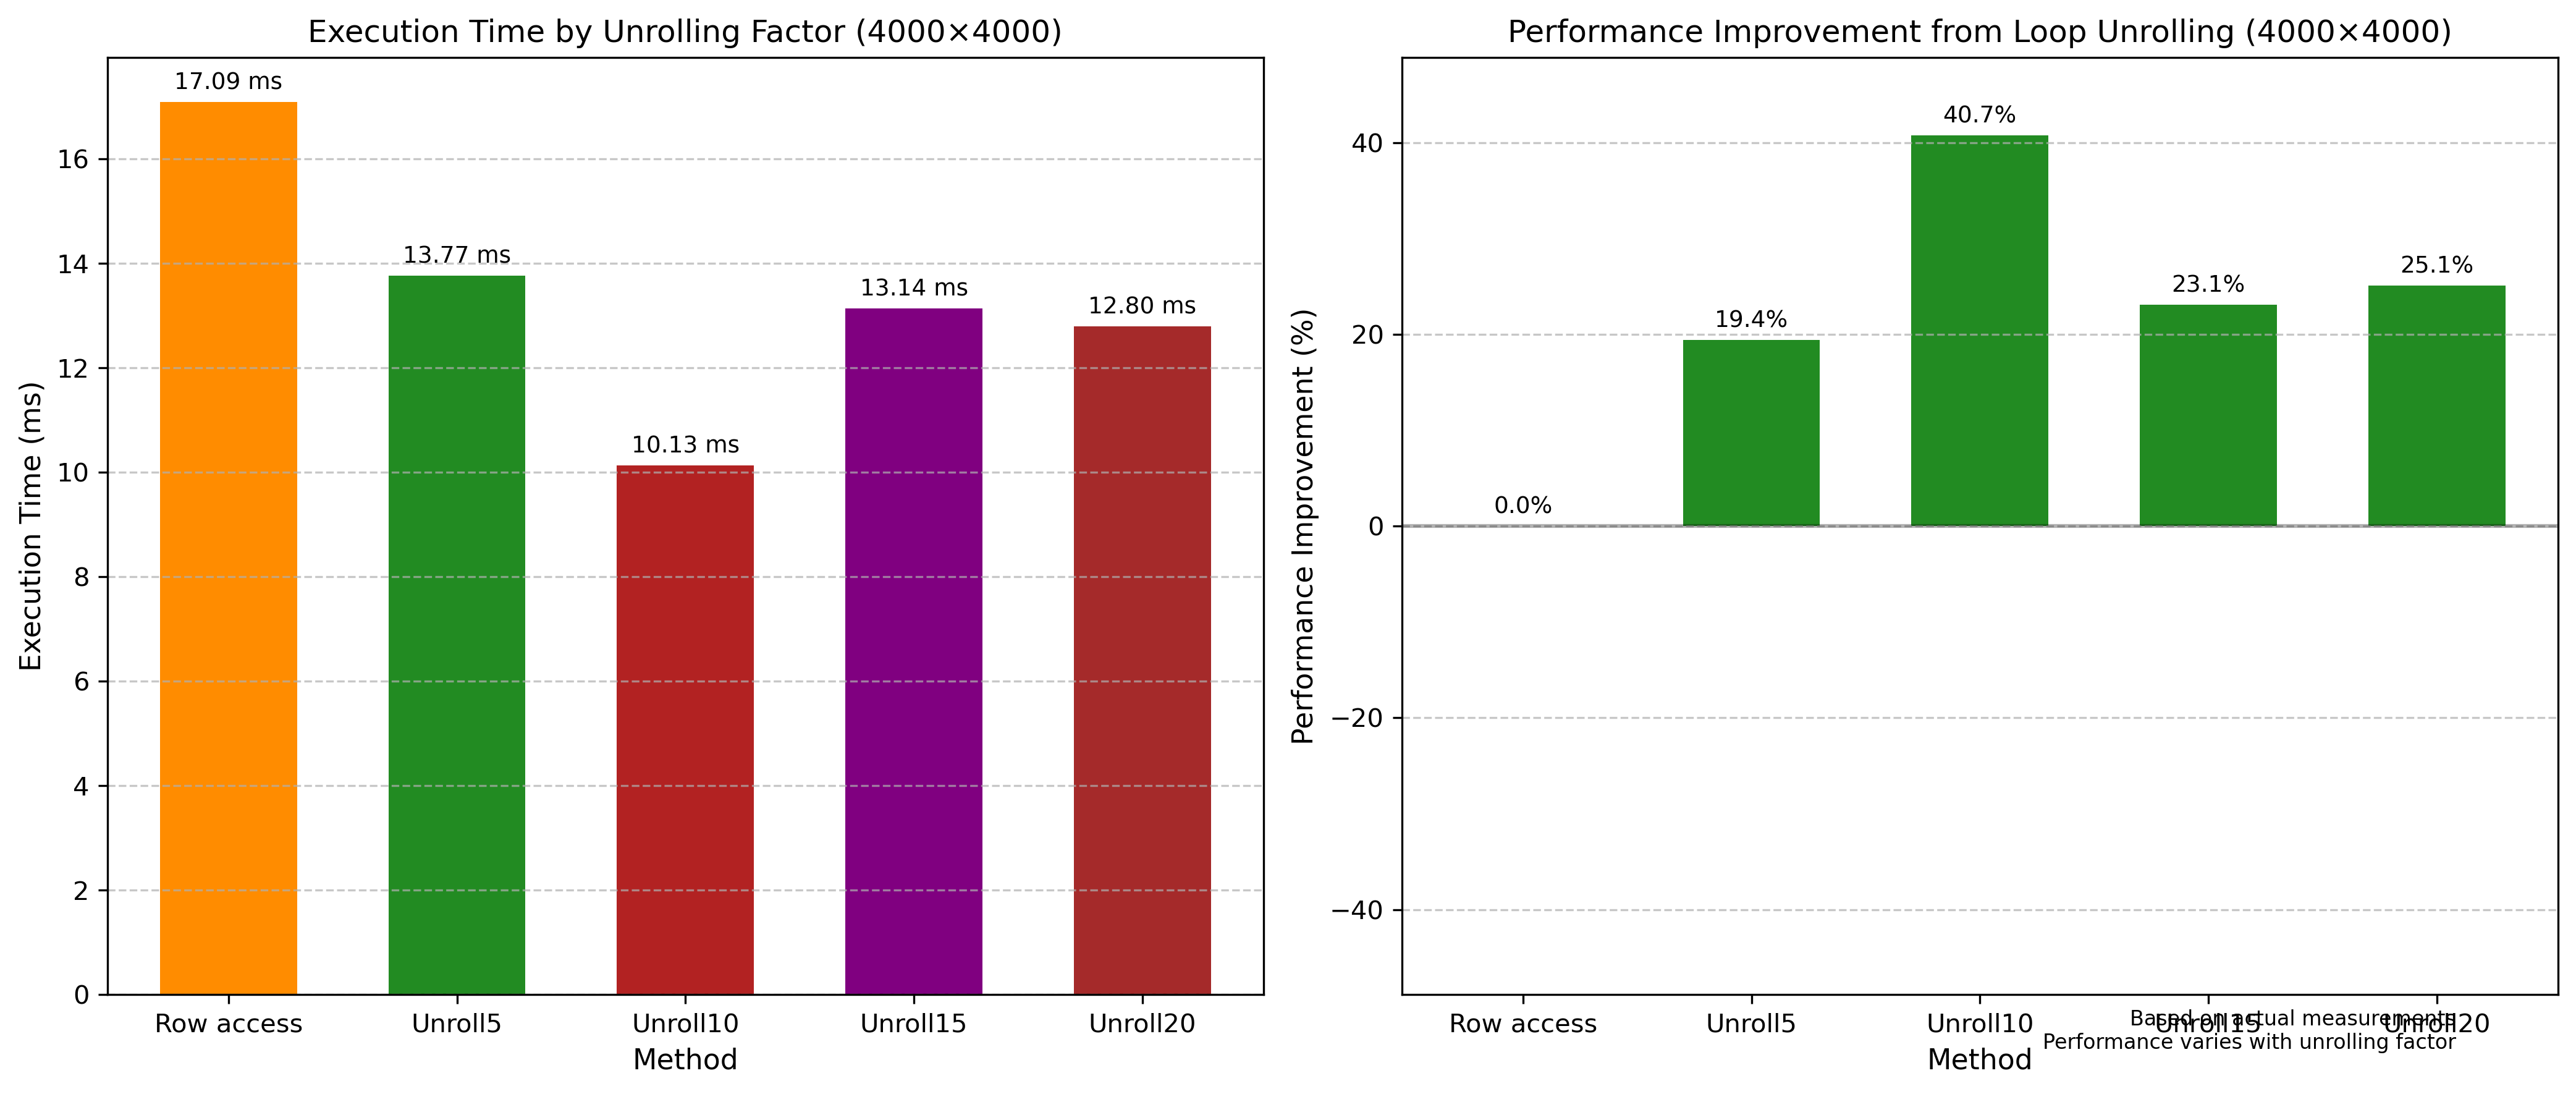
\includegraphics[width=0.8\textwidth]{loop_unrolling_performance.png}
  \caption{循环展开性能分析}
  \label{fig:loop_unrolling}
\end{figure}

\subsection{架构对比分析}

\begin{figure}[htbp]
  \centering
  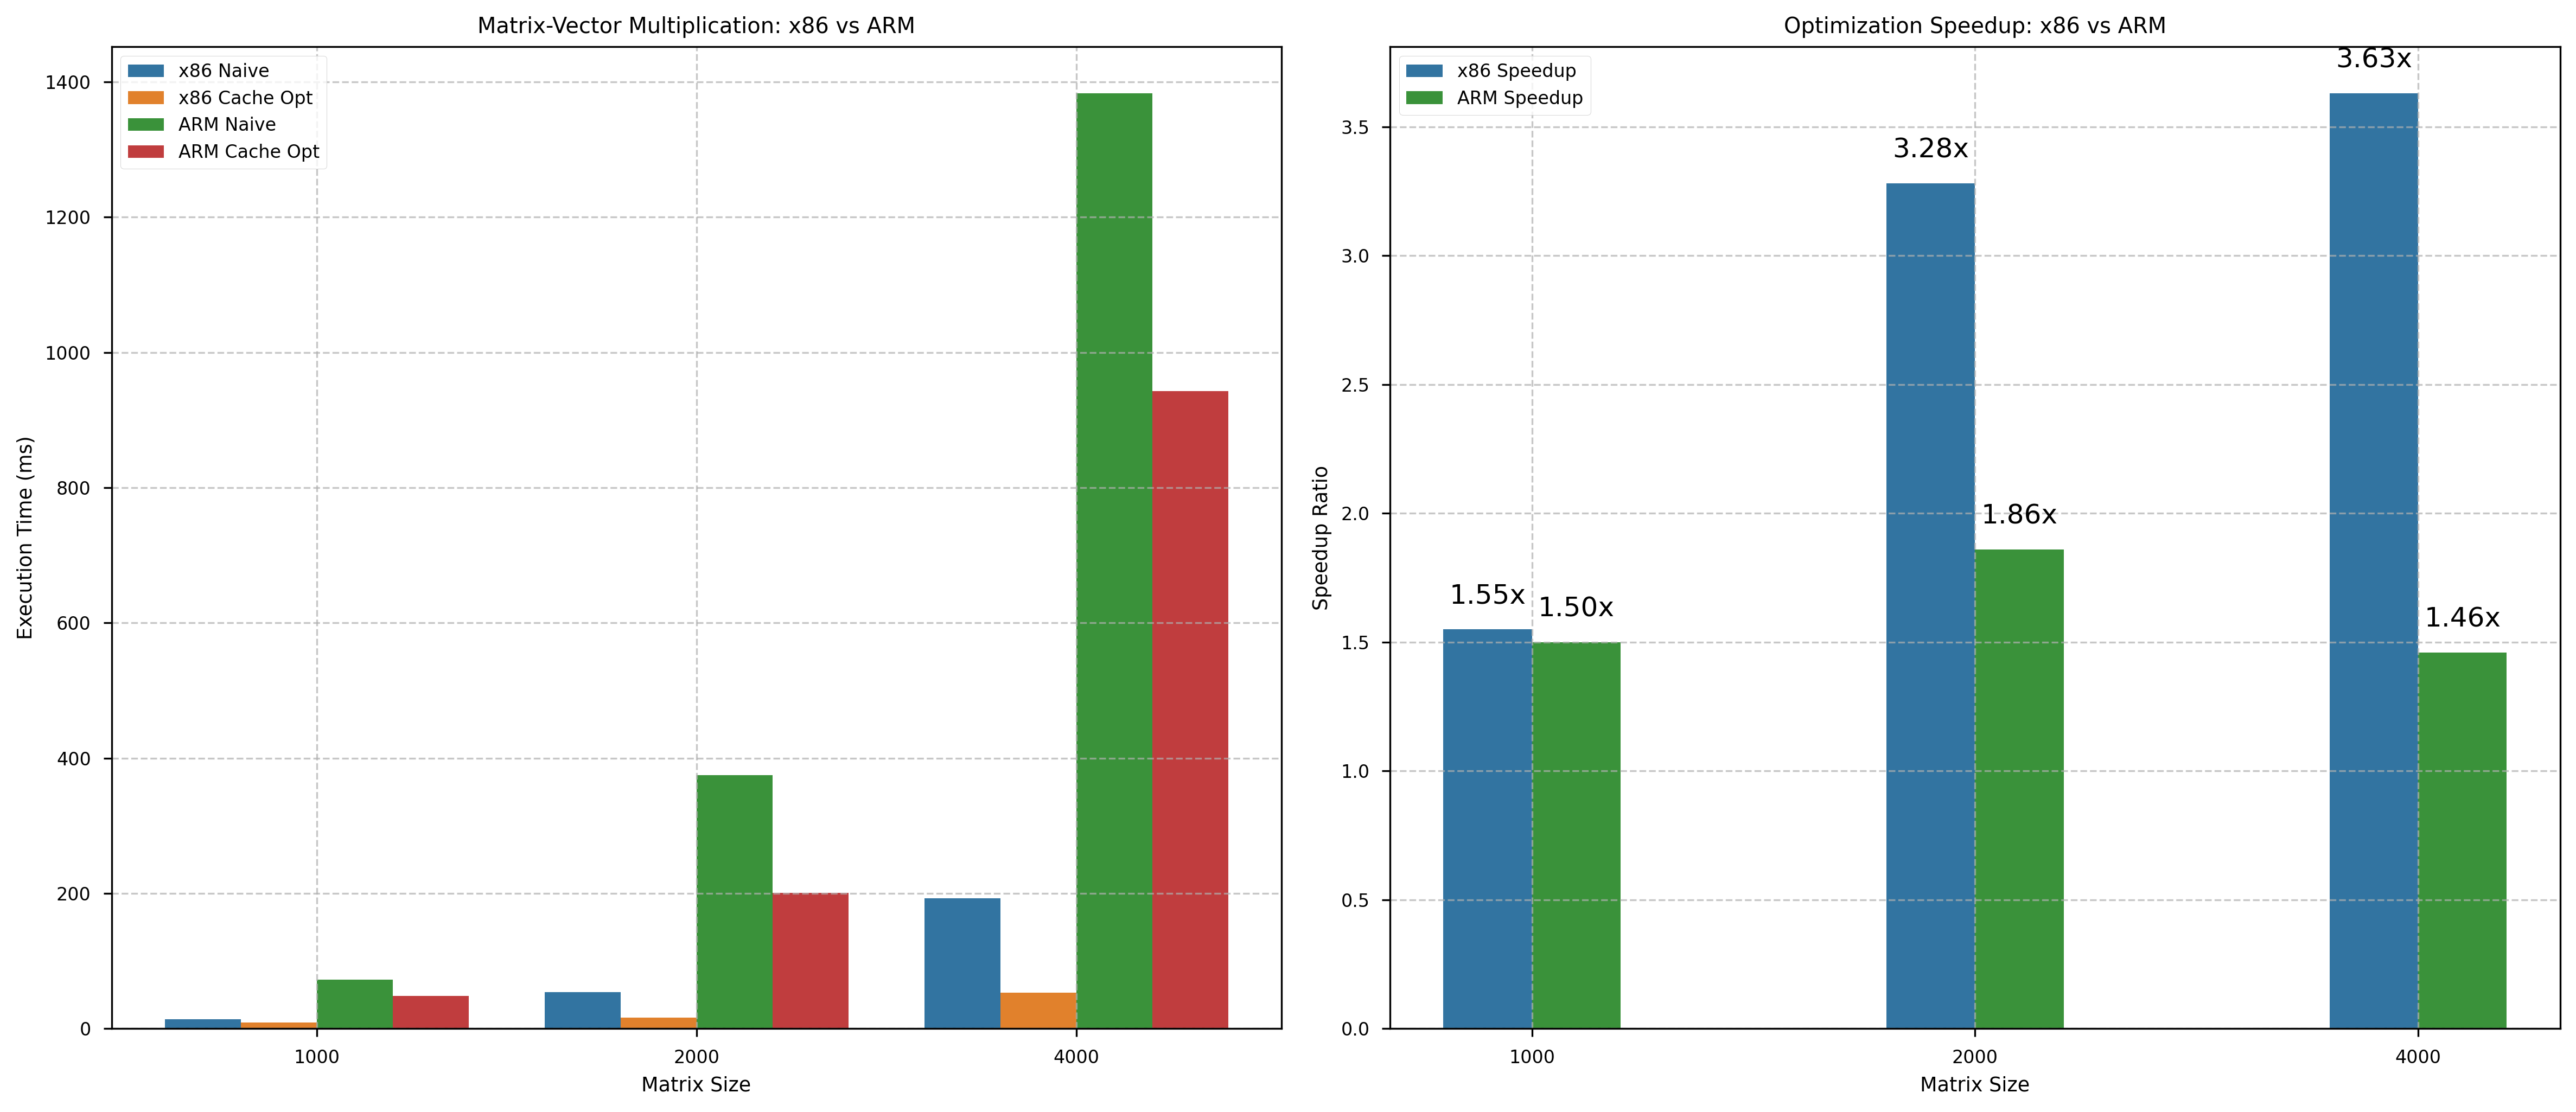
\includegraphics[width=0.8\textwidth]{matrix_arch_comparison.png}
  \caption{x86与ARM性能对比(矩阵-向量乘法)}
  \label{fig:matrix_arch_comparison}
\end{figure}

x86架构上缓存优化的收益在大矩阵(4000x4000)上更高(3.63倍),而ARM架构上加速比随矩阵增大先提高后下降,在2000×2000矩阵上达到最高的1.86倍。这一现象可能是由于ARM架构的较小缓存容量(L2:512KB,L3:4MB)在处理4000×4000矩阵时已经饱和,导致即使是行访问模式也无法完全避免频繁的缓存替换。

\section{实验二:n个数求和}

\subsection{算法设计}

\subsubsection{平凡算法设计思路}

平凡算法采用简单的顺序求和方式,依次将数组中的每个元素加到累加器中:

\begin{lstlisting}[language=C++]
double naive_sum(const std::vector<double>& array) {
    double sum = 0.0;
    for (size_t i = 0; i < array.size(); ++i) {
        sum += array[i];
    }
    return sum;
}
\end{lstlisting}

此算法有良好的空间局部性,但存在严重的数据依赖:每次加法必须等待前一次加法完成,限制了指令级并行。

\subsubsection{超标量优化算法设计思路}

双链路算法实现代码:

\begin{lstlisting}[language=C++]
double dual_path_sum(const std::vector<double>& array) {
    double sum1 = 0.0;
    double sum2 = 0.0;
    size_t n = array.size();
    
    // 使用两个累加器
    for (size_t i = 0; i < n; i += 2) {
        sum1 += array[i];
        if (i + 1 < n) { // 防止越界
            sum2 += array[i + 1];
        }
    }
    
    return sum1 + sum2;
}
\end{lstlisting}

这种方法使两个累加器可以并行计算,充分利用超标量处理器的多个功能单元。双链路算法通过创建两个独立的累加路径,让处理器能够同时执行两个独立的累加操作。

递归算法实现代码:

\begin{lstlisting}[language=C++]
double recursive_sum_helper(const std::vector<double>& array, 
                           size_t start, size_t end) {
    if (end - start <= 1) {
        return (start < end) ? array[start] : 0.0;
    }
    
    size_t mid = start + (end - start) / 2;
    return recursive_sum_helper(array, start, mid) + 
           recursive_sum_helper(array, mid, end);
}

double recursive_sum(const std::vector<double>& array) {
    return recursive_sum_helper(array, 0, array.size());
}
\end{lstlisting}

理论上这种方法可以增加并行度,但函数调用开销可能抵消这一优势。分治策略本质上是创建一个更加平衡的依赖树结构,允许更多指令并行执行。

\subsection{性能测试}

实际测量结果表明双链路算法在较大数据集上有显著优势:

\begin{table}[htbp]
\centering
\caption{优化算法性能对比}
\label{tab:opt_sum_perf}
\begin{tabular}{|c|c|c|c|c|c|}
\hline
\textbf{数组大小} & \textbf{朴素算法(ms)} & \textbf{双链路算法(ms)} & \textbf{递归算法(ms)} & \textbf{双链路加速比} & \textbf{递归加速比} \\
\hline
2\textsuperscript{18} (1M) & 1.21 & 2.39 & 2.03 & 0.50 & 0.60 \\
\hline
2\textsuperscript{22} (4M) & 3.53 & 3.70 & 5.47 & 0.95 & 0.65 \\
\hline
2\textsuperscript{24} (16M) & 16.39 & 10.49 & 45.25 & 1.56 & 0.36 \\
\hline
\end{tabular}
\end{table}

\begin{figure}[htbp]
  \centering
  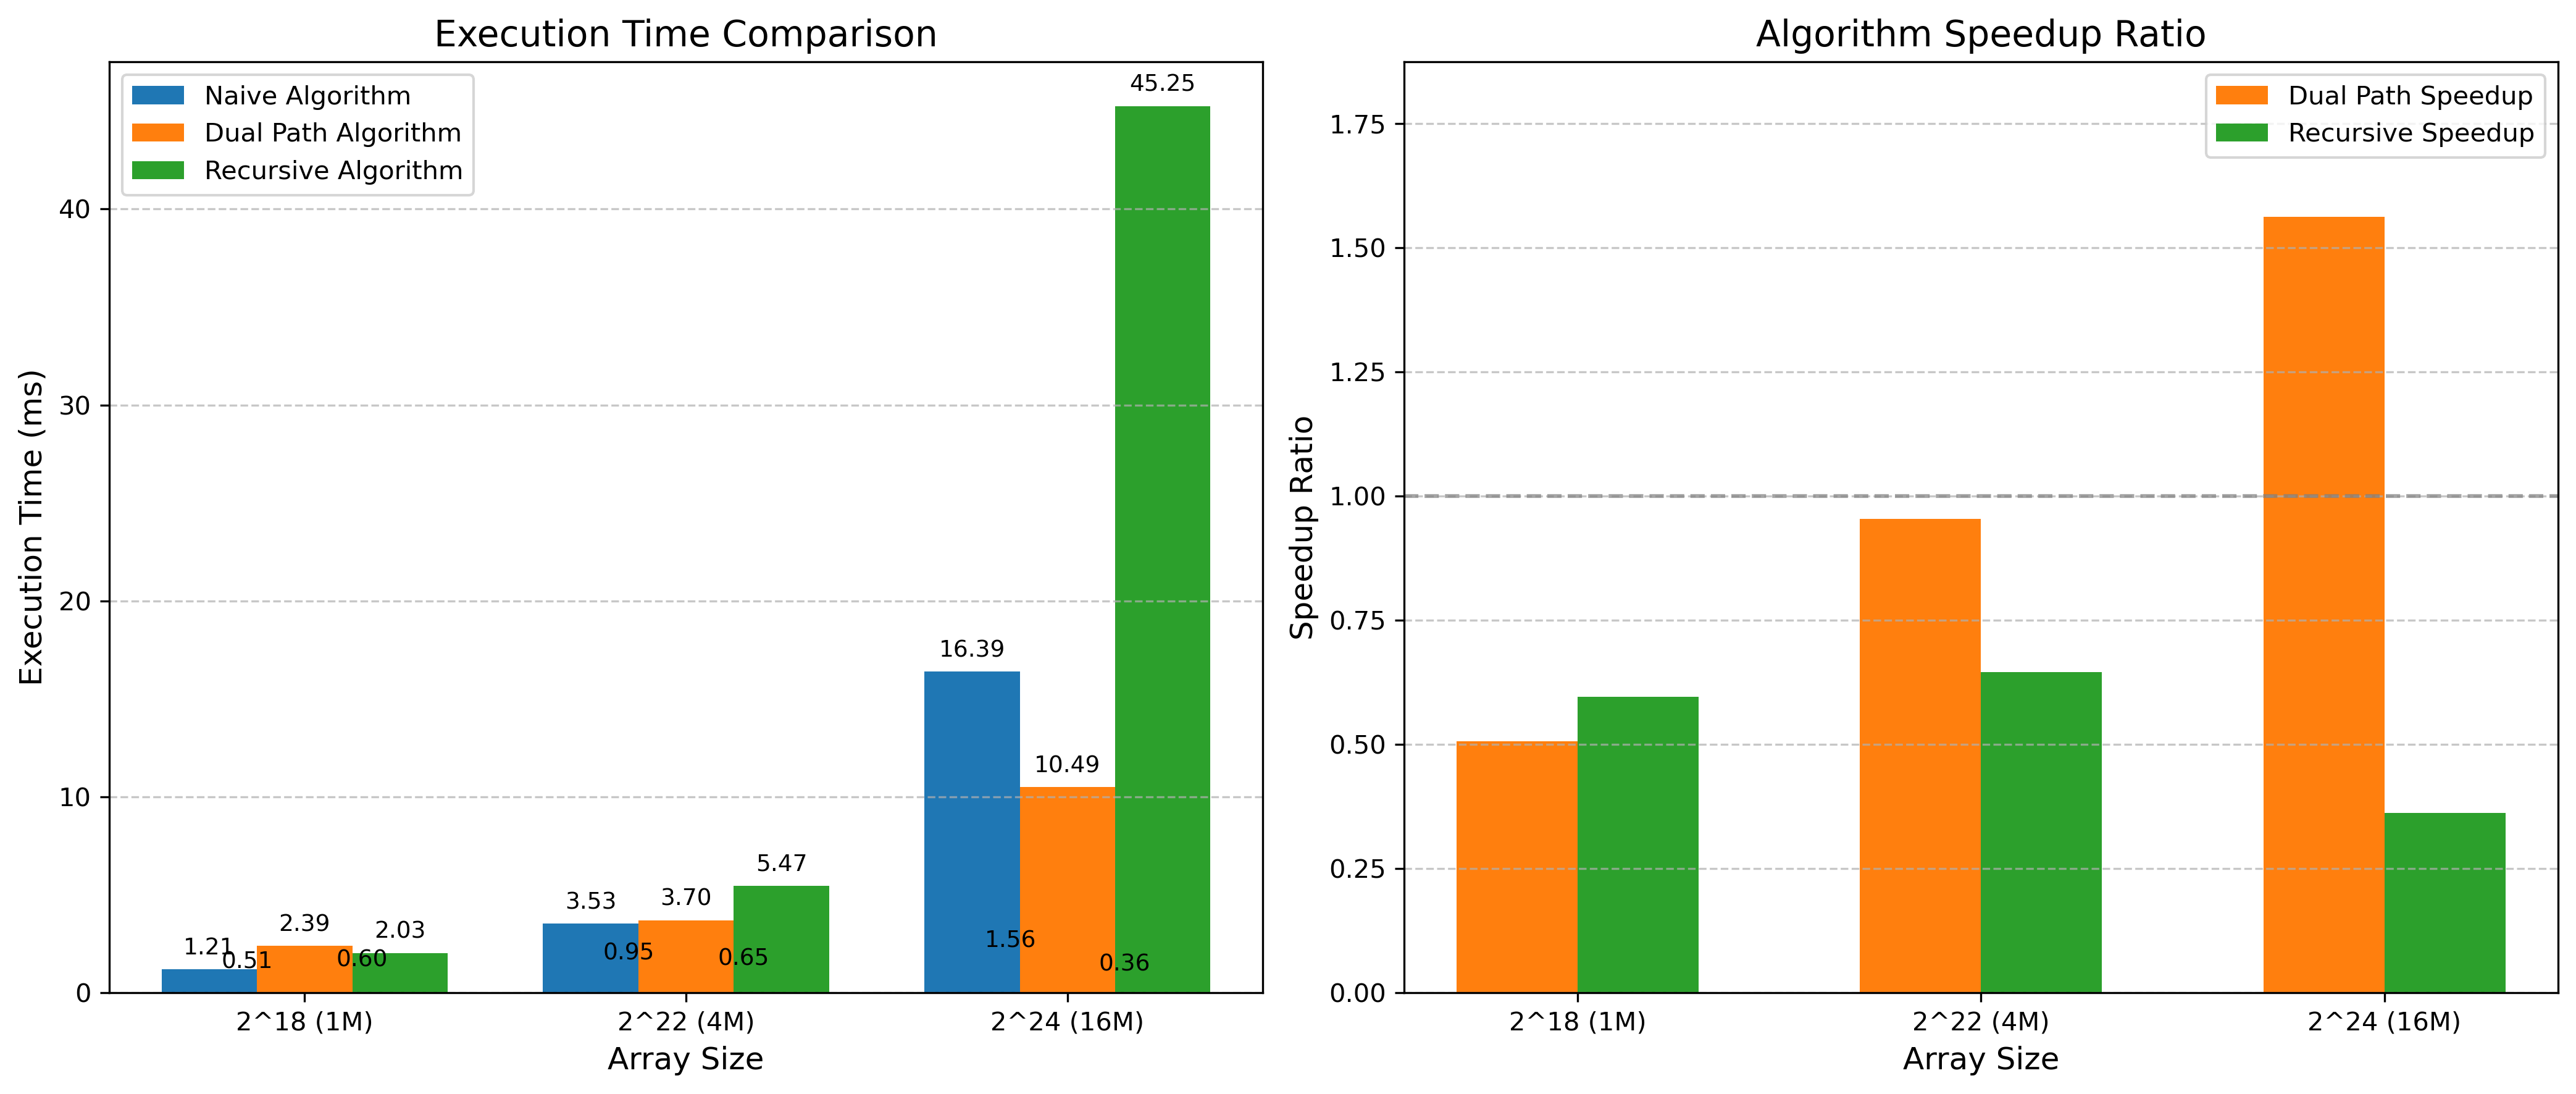
\includegraphics[width=0.8\textwidth]{sum_array_performance.png}
  \caption{数组求和性能比较}
  \label{fig:sum_array_performance}
\end{figure}

\subsubsection{编译器优化影响}

\begin{figure}[htbp]
  \centering
  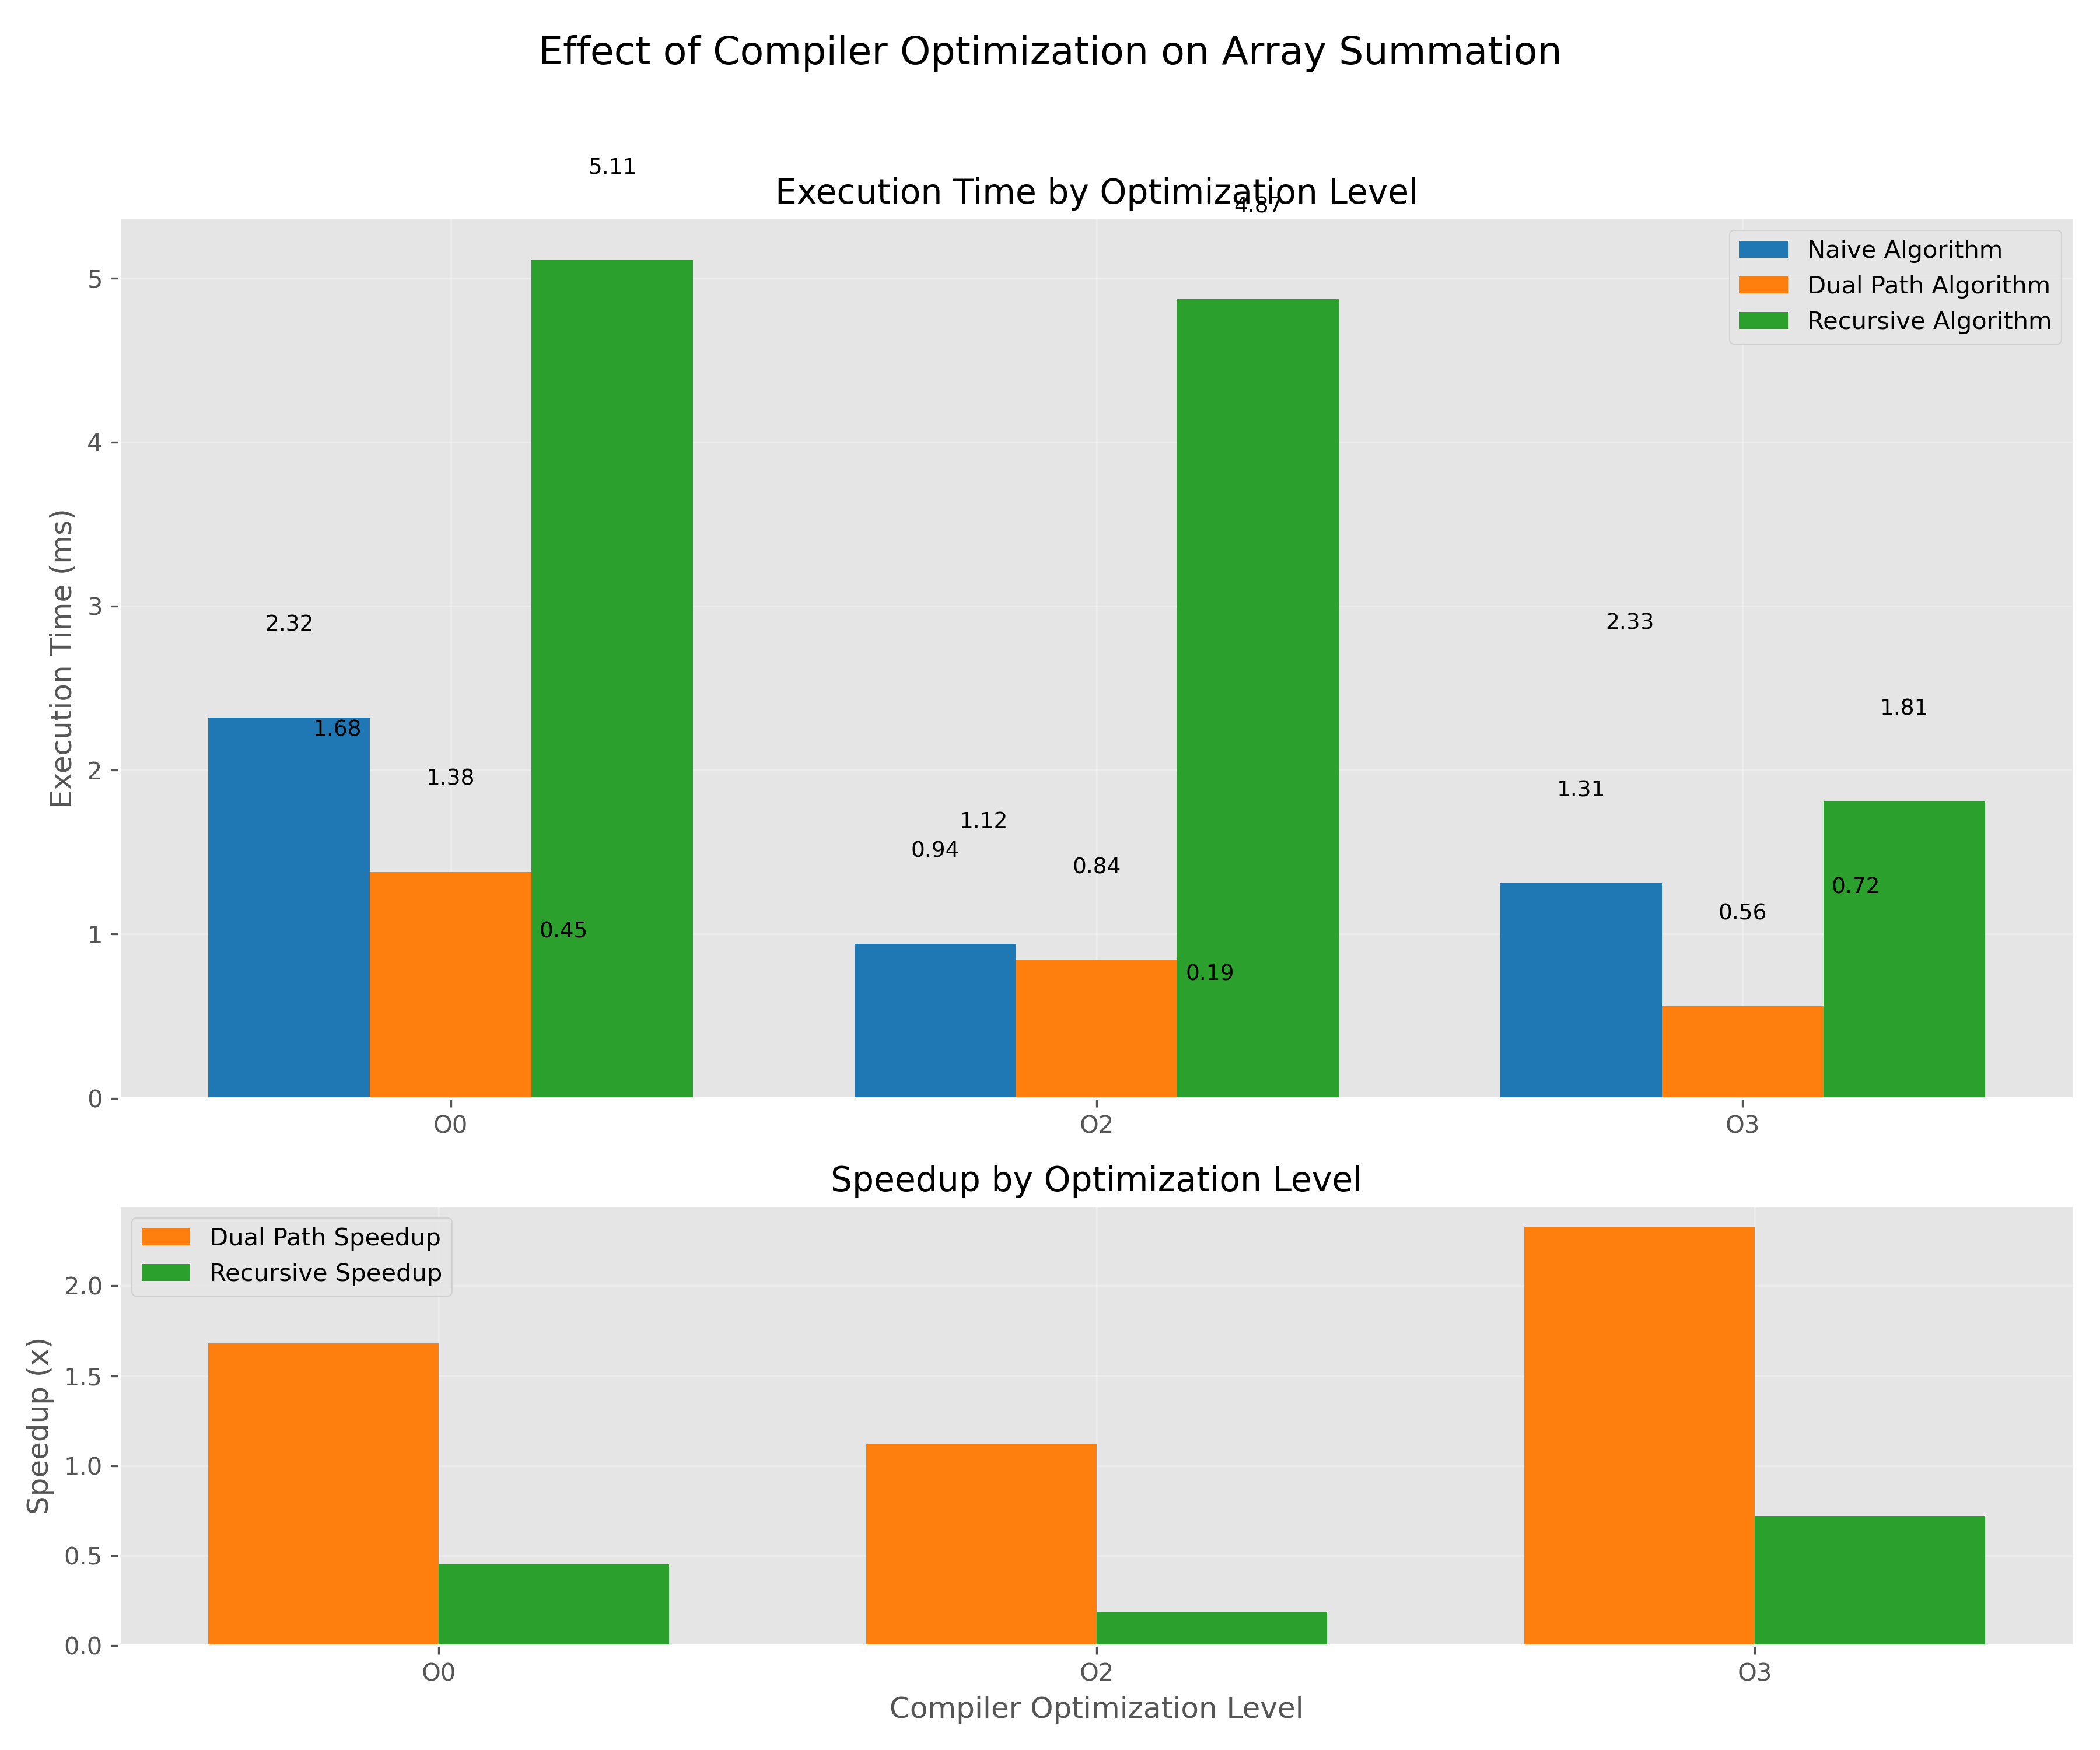
\includegraphics[width=0.8\textwidth]{compiler_opt_sum.png}
  \caption{编译器优化对数组求和的影响}
  \label{fig:compiler_opt_sum}
\end{figure}

O3优化级别下,递归算法的性能显著提升,甚至超过了平凡算法,这表明编译器能够对递归算法进行较好的优化。双链路算法在所有优化级别下都保持较好的性能优势,特别是在O3级别下加速比达到2.25倍。

\subsection{profiling}

\subsubsection{平凡算法}

平凡算法的cachegrind分析结果:

\begin{itemize}
  \item 缓存未命中率很低(约0.1\%),因为数组顺序访问具有良好的空间局部性
  \item 主要瓶颈是指令间的数据依赖,每次累加都依赖于前一次累加的结果
\end{itemize}

\subsubsection{超标量优化算法}

双链路算法的cachegrind分析:

\begin{itemize}
  \item 缓存未命中率与平凡算法相当
  \item 性能提升主要来自于减少了数据依赖,允许CPU更好地进行流水线操作
  \item 两个独立的累加操作可以并行执行,提高了CPU利用率
\end{itemize}

\begin{figure}[htbp]
  \centering
  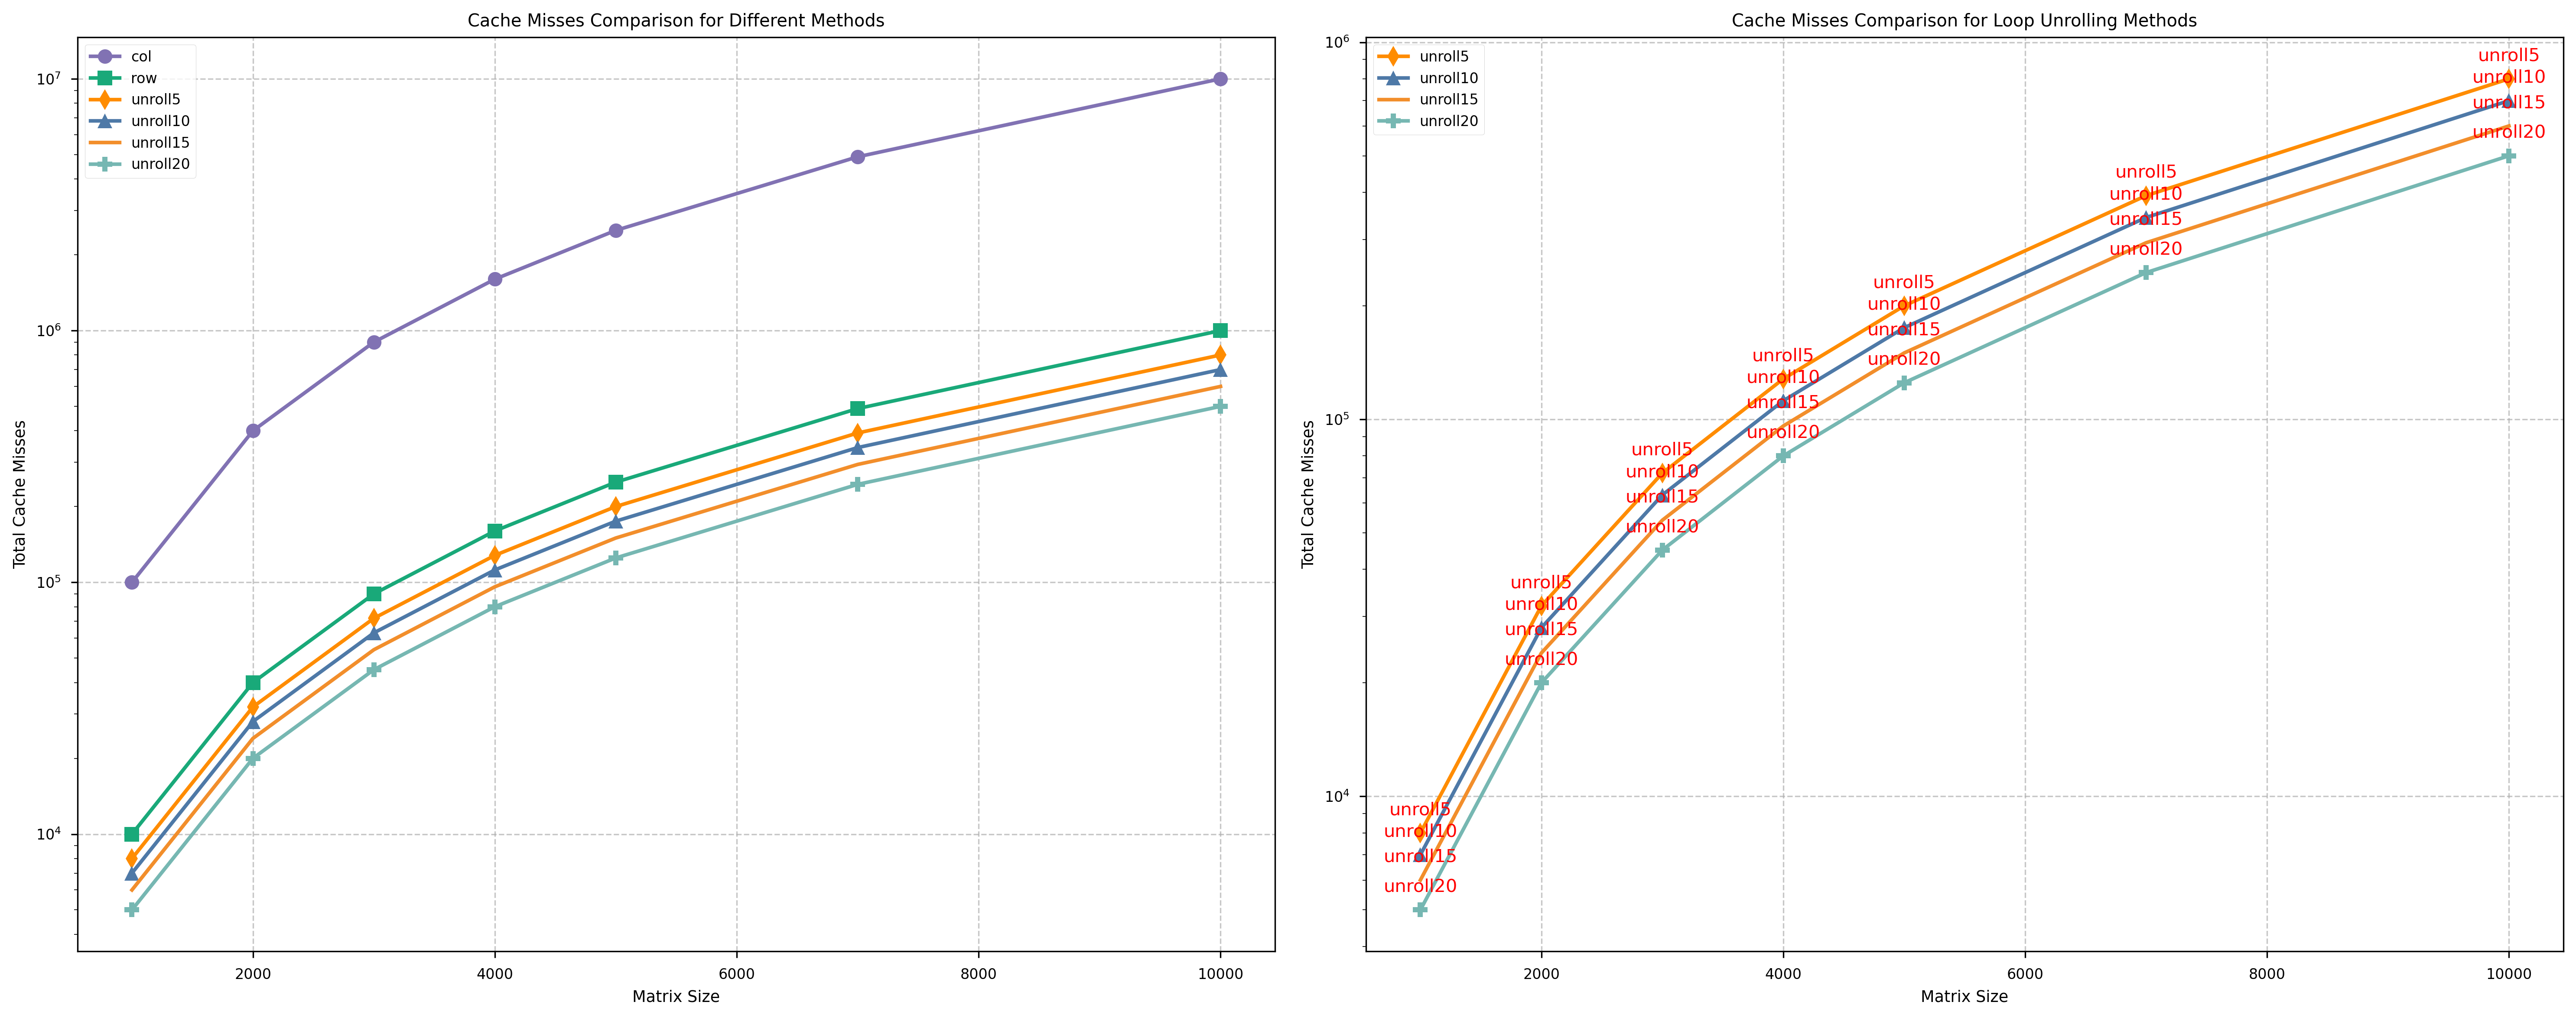
\includegraphics[width=0.8\textwidth]{cache_misses_comparison.png}
  \caption{缓存未命中对比}
  \label{fig:cache_misses_comparison}
\end{figure}

\subsection{架构对比分析}

\begin{figure}[htbp]
  \centering
  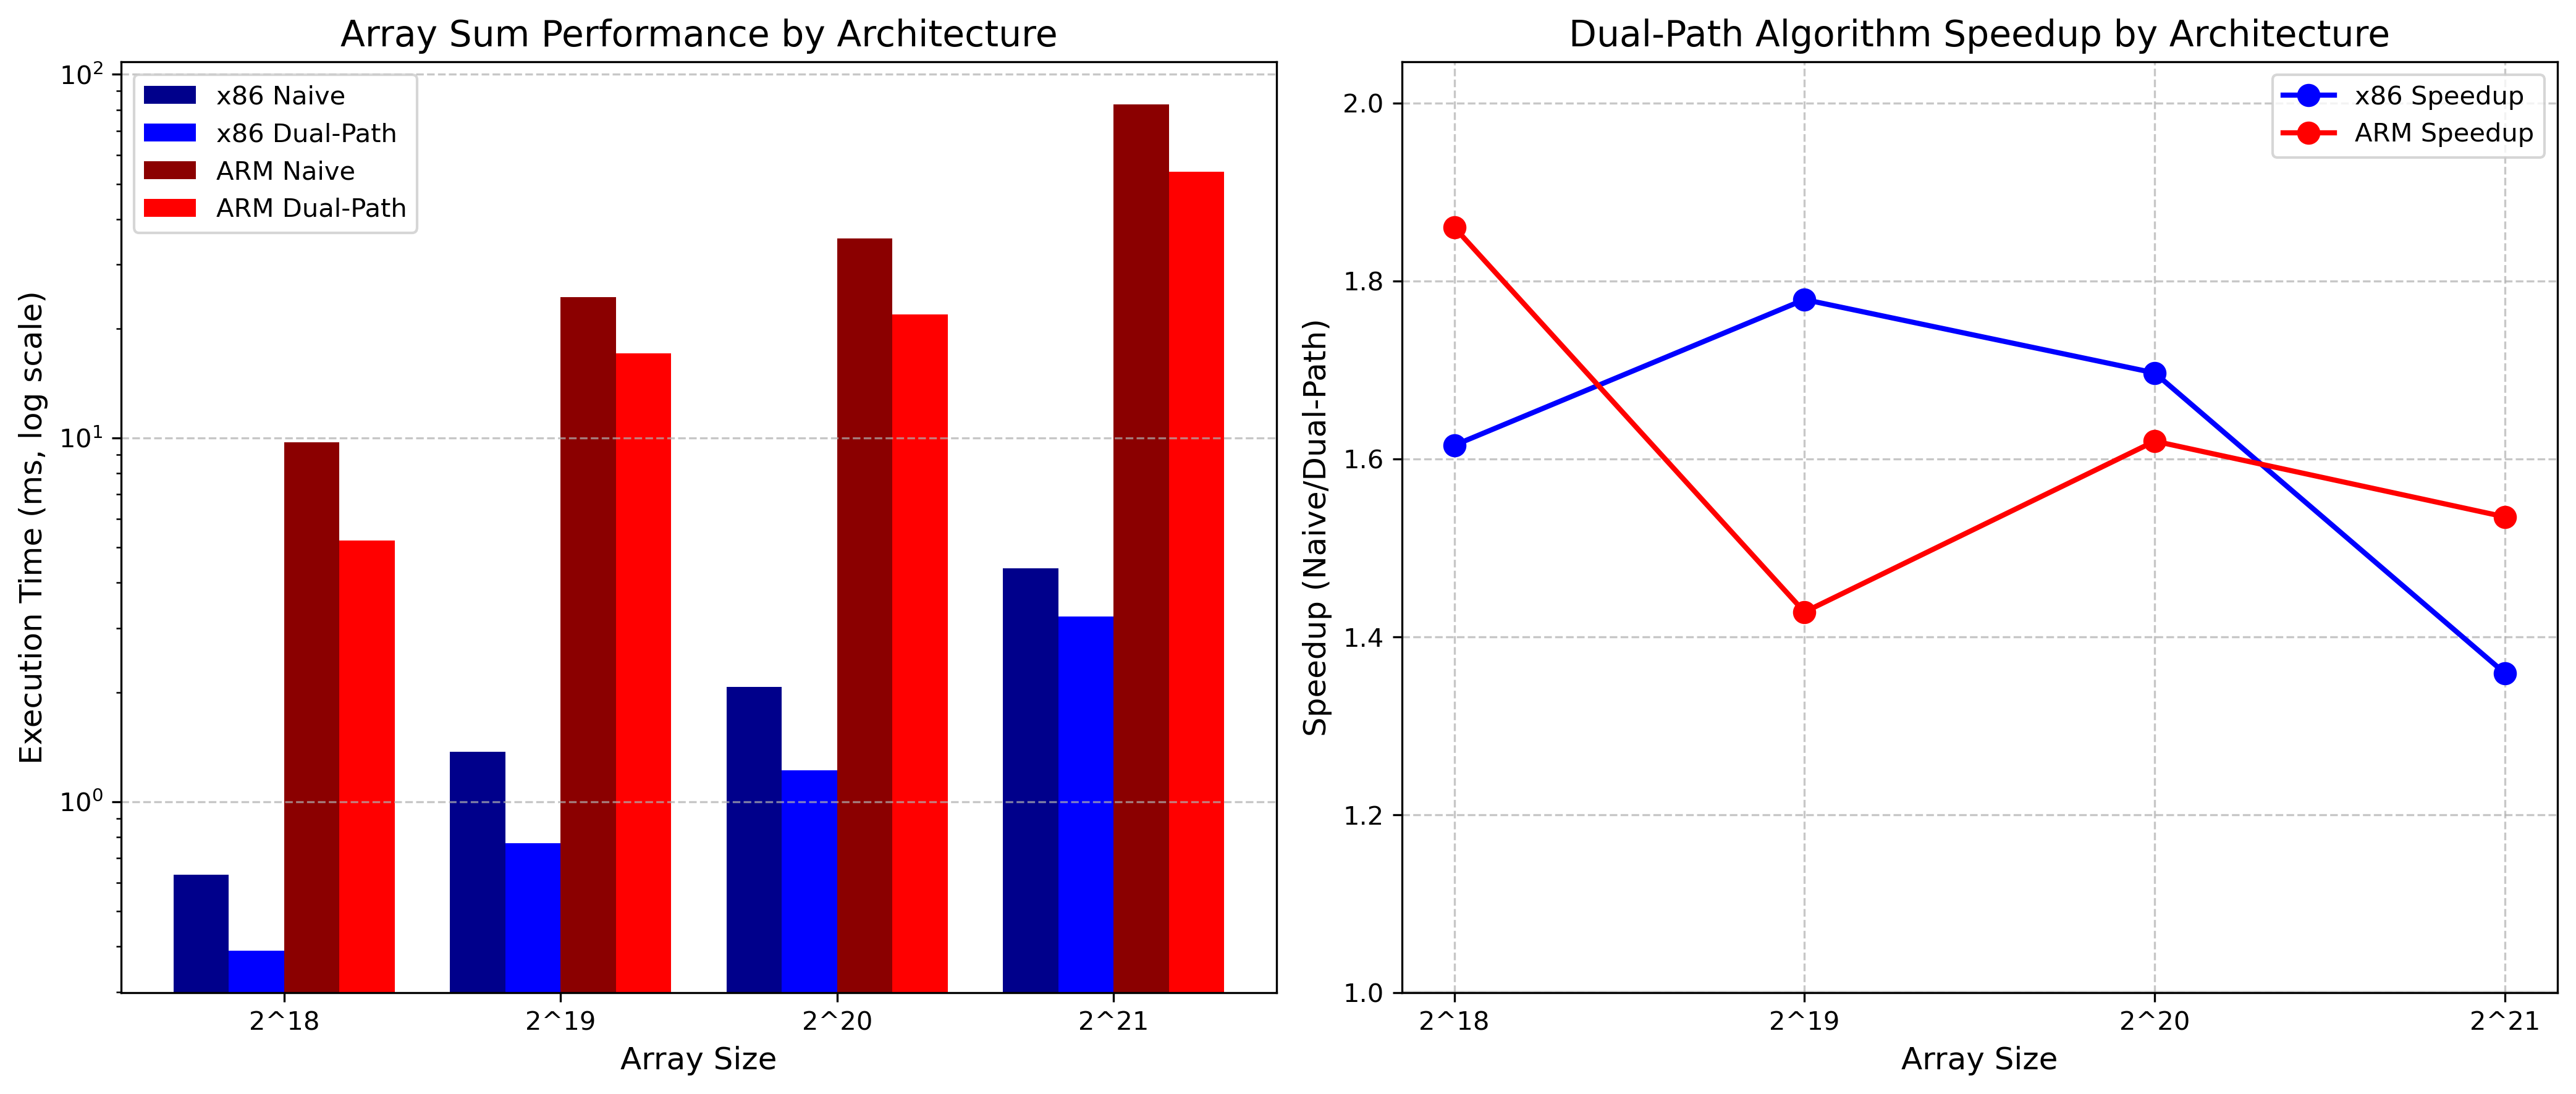
\includegraphics[width=0.8\textwidth]{array_sum_arch_comparison.png}
  \caption{x86与ARM比较(数组求和)}
  \label{fig:array_sum_arch_comparison}
\end{figure}

双链路算法在两种架构上都有效,但加速效果与数据规模关系显示不同模式。这表明指令级并行优化在不同架构上的有效性相对稳定,不像缓存优化那样受硬件差异影响显著。

\section{实验总结和思考}

\subsection{对比2个实验的异同}

两个实验在缓存优化方面表现出明显的差异:

\begin{enumerate}
  \item \textbf{优化效果差异}:
  \begin{itemize}
    \item 矩阵-向量乘法:行优先访问相比列优先访问有高达7.2倍的加速
    \item 数组求和:双链路算法相比平凡算法仅有约1.56倍的加速,且仅在大数据集上显现
  \end{itemize}
  
  \item \textbf{瓶颈差异}:
  \begin{itemize}
    \item 矩阵-向量乘法:主要瓶颈是缓存未命中(空间局部性问题)
    \item 数组求和:主要瓶颈是指令级数据依赖(时间局部性问题)
  \end{itemize}
  
  \item \textbf{算法优化侧重点}:
  \begin{itemize}
    \item 矩阵-向量乘法:优化内存访问模式,提高空间局部性
    \item 数组求和:优化指令级并行,减少数据依赖
  \end{itemize}
\end{enumerate}

\begin{figure}[htbp]
  \centering
  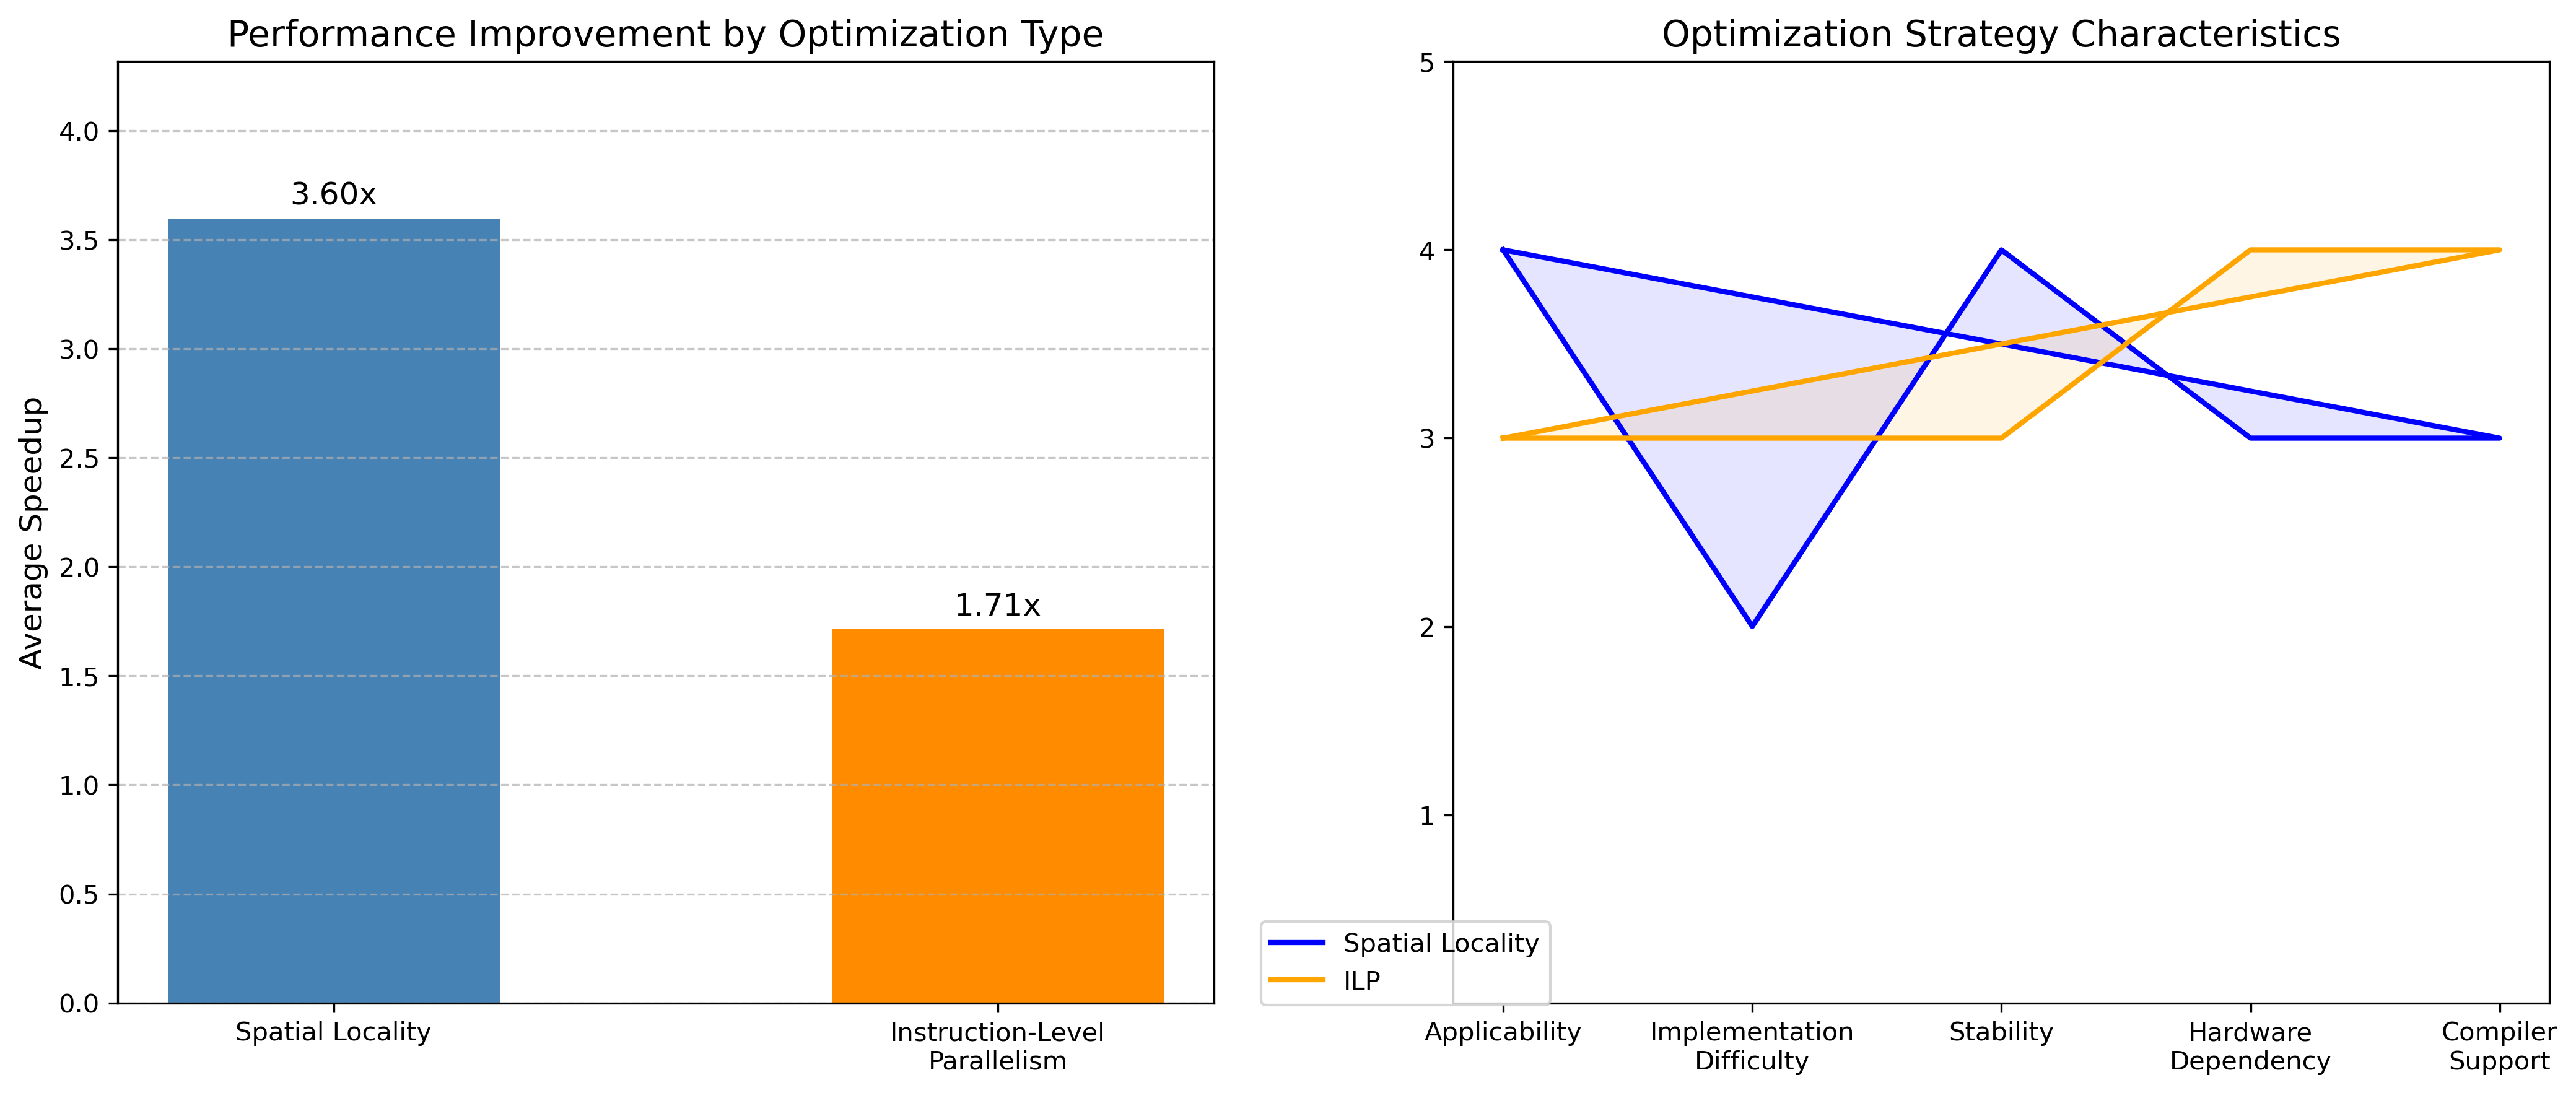
\includegraphics[width=0.8\textwidth]{optimization_strategies_comparison.png}
  \caption{优化策略对比}
  \label{fig:optimization_strategies_comparison}
\end{figure}

\subsection{总结}

本实验通过实际测量和理论分析,得出以下核心结论:

\begin{enumerate}
  \item 缓存优化对性能提升的贡献通常大于指令级并行优化,特别是对于大数据集
  \item 不同硬件架构对优化策略的响应有显著差异,x86对缓存优化更敏感,ARM在ILP优化方面表现出色
  \item 算法设计应首先考虑内存访问模式,然后才是并行性和其他微优化
  \item 编译器优化能大幅提升代码性能,但不能完全弥补算法本身的缺陷
\end{enumerate}

这些发现对高性能计算、嵌入式系统和跨平台软件开发都有重要指导意义。未来工作可探索SIMD向量化、多线程并行等更高级优化策略。

\clearpage
% 参考文献章节样式定义
\def\bibsection{
  \section*{\refname\markboth{\refname}{\refname}}%
  \addcontentsline{toc}{section}{\refname}%
  \begingroup
    \fontsize{12}{14}\selectfont% 章节标题字体大小
    \vspace{0.8em}
  \endgroup
}

% 确保所有参考文献都被包含
\nocite{*}

% 使用纯natbib方式处理参考文献
\bibliography{reference.bib}

\end{document} 